\chapter{An Introduction to R}






\begin{quote}
\emph{This is a lightly modified version of a handout RJP used with his 
Intro Stats students Spring 2011.  Aside from the occasional comment to
instructors, this chapter could be used essentially as is with students.}
\end{quote}

\label{app:StartingR}

\section{Welcome to \R\ and \Rstudio}

\R\ is a system for statistical computation and graphics.  We use \R\ for several reasons:
\begin{enumerate}
\item \R\ is open-source and freely available for Mac, PC, and Linux machines.
This means that there is no restriction on having to license a particular
software program, or have
students work in a specific lab that has been outfitted with the technology of choice.
\item \R\ is user-extensible and user extensions can easily be made available to others.
\item \R\ is commercial quality.  It is the package of choice for many statisticians and those
who use statistics frequently.  
\item \R\ is becoming very popular with statisticians and scientists, especially in certain
sub-disciplines, like genetics.  Articles in research journals such as \textit{Science} often
include links to the \R\ code used for the analysis and graphics presented.
\item
\R\ is very powerful.  Furthermore, it is gaining new features every day.  New statistical 
methods are often available first in \R.
\end{enumerate}

\Rstudio\ provides access to \R\ in a web browser.  This has some additional
advantages: no installation is required, the interface has some additional user-friendly components,
and work begun on one machine can be picked up seamlessly later on somewhere else.

The URL for the \RStudio\ beta server is
\begin{center}
\url{http://beta.rstudio.org/}
\end{center}

It is also possible to download \RStudio\ server and set up your own server or \RStudio\ desktop
for stand-alone processing.


%You should be able to log in using the Gmail address that you provided earlier.
Once you have logged in to an \RStudio\ server, you will see something like Figure~\ref{fig:Rstudio-bigview}.

\begin{figure}
\begin{center}
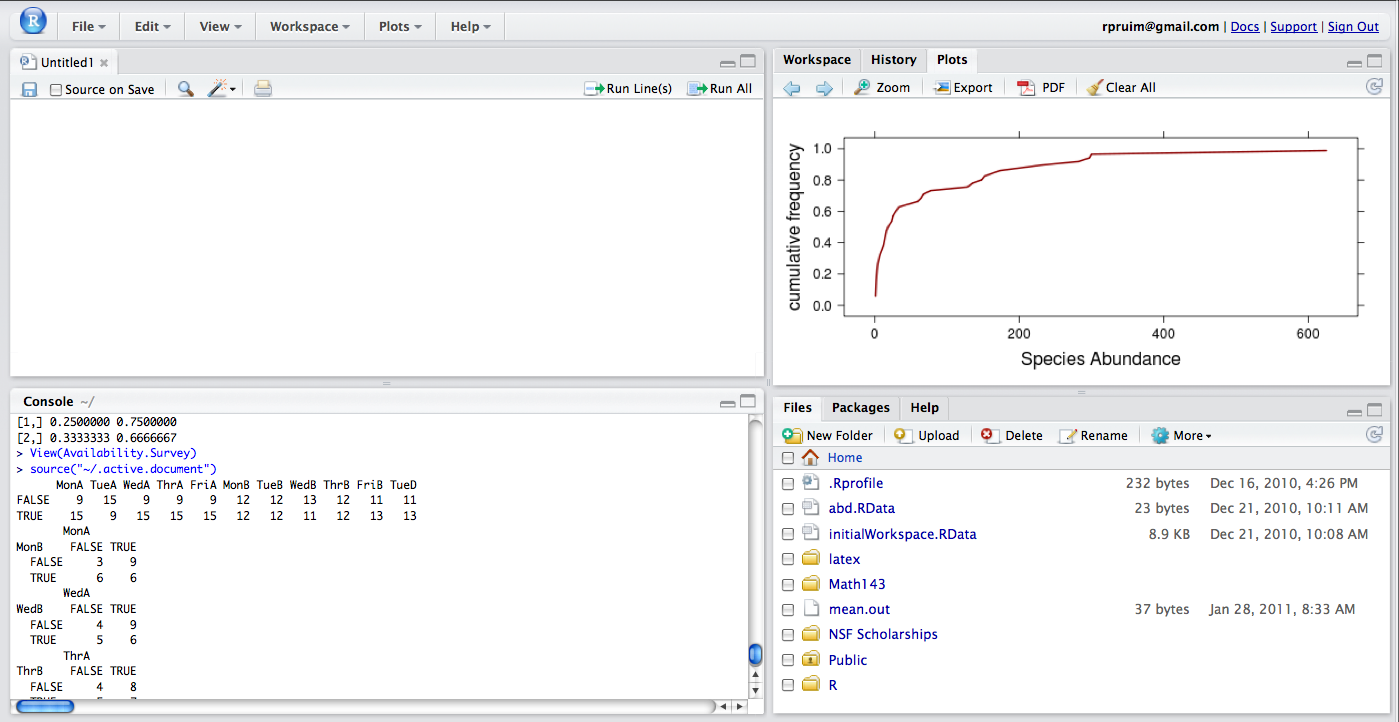
\includegraphics[width=1.0\textwidth]{images/RStudio-bigview}
\end{center}
\caption{Welcome to \Rstudio.}
\label{fig:Rstudio-bigview}%
\end{figure}

Notice that \Rstudio\ divides its world into four panels.  Several of the panels
are further subdivided into multiple tabs.
The console panel is where we type commands that \R\ will execute. 

\begin{problem}
Calculate the natural logarithm (log base $e$) and base 10 logarithm of 12,345.

What happens if you leave the comma in this number?
\begin{knitrout}
\definecolor{shadecolor}{rgb}{.97, .97, .97}{\color{fgcolor}\begin{kframe}
\begin{flushleft}
\ttfamily\noindent
\hlfunctioncall{log}\hlkeyword{(}\hlnumber{12}\hlkeyword{,}{\ }\hlnumber{345}\hlkeyword{)}\mbox{}
\normalfont
\end{flushleft}
\begin{verbatim}
[1] 0.4252
\end{verbatim}
\end{kframe}}
\end{knitrout}

%Copy-and-paste your \R\ code into your Word document.  
%Be sure to use a fixed-width font (like Courier) when you display \R\ code.  This will
%(1) make it clear that you are displaying \R\ input or output, and (2) keep things aligned 
%properly.
\end{problem}

%\pagebreak
\section{Using R as a Calculator}
\R\ can be used as a calculator.  Try typing the following commands in the console panel.

\begin{knitrout}
\definecolor{shadecolor}{rgb}{.97, .97, .97}{\color{fgcolor}\begin{kframe}
\begin{flushleft}
\ttfamily\noindent
\hlnumber{5}{\ }\hlkeyword{+}{\ }\hlnumber{3}\mbox{}
\normalfont
\end{flushleft}
\begin{verbatim}
[1] 8
\end{verbatim}
\begin{flushleft}
\ttfamily\noindent
\hlnumber{15.3}{\ }\hlkeyword{*}{\ }\hlnumber{23.4}\mbox{}
\normalfont
\end{flushleft}
\begin{verbatim}
[1] 358
\end{verbatim}
\begin{flushleft}
\ttfamily\noindent
\hlfunctioncall{sqrt}\hlkeyword{(}\hlnumber{16}\hlkeyword{)}\mbox{}
\normalfont
\end{flushleft}
\begin{verbatim}
[1] 4
\end{verbatim}
\end{kframe}}
\end{knitrout}

You can save values to named variables for later reuse.
\TeachingTip{It's probably best to settle on using 
one or the other of the right-to-left assignment operators rather than to switch
back and forth.  The authors of this document have different preferences.}%

\begin{knitrout}
\definecolor{shadecolor}{rgb}{.97, .97, .97}{\color{fgcolor}\begin{kframe}
\begin{flushleft}
\ttfamily\noindent
\hlsymbol{product}{\ }\hlassignement{=}{\ }\hlnumber{15.3}{\ }\hlkeyword{*}{\ }\hlnumber{23.4}{\ }{\ }\hlcomment{\usebox{\hlnormalsizeboxhash}{\ }save{\ }result}\hspace*{\fill}\\
\hlstd{}\hlsymbol{product}{\ }{\ }\hlcomment{\usebox{\hlnormalsizeboxhash}{\ }show{\ }the{\ }result}\mbox{}
\normalfont
\end{flushleft}
\begin{verbatim}
[1] 358
\end{verbatim}
\begin{flushleft}
\ttfamily\noindent
\hlsymbol{product}{\ }\hlassignement{\usebox{\hlnormalsizeboxlessthan}-}{\ }\hlnumber{15.3}{\ }\hlkeyword{*}{\ }\hlnumber{23.4}{\ }{\ }\hlcomment{\usebox{\hlnormalsizeboxhash}{\ }\usebox{\hlnormalsizeboxlessthan}-{\ }is{\ }assignment{\ }operator,{\ }same{\ }as{\ }=}\hspace*{\fill}\\
\hlstd{}\hlsymbol{product}\mbox{}
\normalfont
\end{flushleft}
\begin{verbatim}
[1] 358
\end{verbatim}
\begin{flushleft}
\ttfamily\noindent
\hlsymbol{newproduct}{\ }{\ }\hlcomment{\usebox{\hlnormalsizeboxhash}{\ }-\usebox{\hlnormalsizeboxgreaterthan}{\ }assigns{\ }to{\ }the{\ }right{\ }\usebox{\hlnormalsizeboxlessthan}-{\ }15.3{\ }*{\ }}\mbox{}
\normalfont
\end{flushleft}
\begin{verbatim}
Error: object 'newproduct' not found
\end{verbatim}
\begin{flushleft}
\ttfamily\noindent
{\ }{\ }{\ }{\ }\hlnumber{23.4}\mbox{}
\normalfont
\end{flushleft}
\begin{verbatim}
[1] 23.4
\end{verbatim}
\begin{flushleft}
\ttfamily\noindent
\hlsymbol{newproduct}\mbox{}
\normalfont
\end{flushleft}
\begin{verbatim}
Error: object 'newproduct' not found
\end{verbatim}
\end{kframe}}
\end{knitrout}

Once variables are defined, they can be referenced with other operators
and functions.

\begin{knitrout}
\definecolor{shadecolor}{rgb}{.97, .97, .97}{\color{fgcolor}\begin{kframe}
\begin{flushleft}
\ttfamily\noindent
\hlnumber{0.5}{\ }\hlkeyword{*}{\ }\hlsymbol{product}{\ }{\ }\hlcomment{\usebox{\hlnormalsizeboxhash}{\ }half{\ }of{\ }the{\ }product}\mbox{}
\normalfont
\end{flushleft}
\begin{verbatim}
[1] 179
\end{verbatim}
\begin{flushleft}
\ttfamily\noindent
\hlfunctioncall{log}\hlkeyword{(}\hlsymbol{product}\hlkeyword{)}{\ }{\ }\hlcomment{\usebox{\hlnormalsizeboxhash}{\ }(natural){\ }log{\ }of{\ }the{\ }product}\mbox{}
\normalfont
\end{flushleft}
\begin{verbatim}
[1] 5.881
\end{verbatim}
\begin{flushleft}
\ttfamily\noindent
\hlfunctioncall{log10}\hlkeyword{(}\hlsymbol{product}\hlkeyword{)}{\ }{\ }\hlcomment{\usebox{\hlnormalsizeboxhash}{\ }base{\ }10{\ }log{\ }of{\ }the{\ }product}\mbox{}
\normalfont
\end{flushleft}
\begin{verbatim}
[1] 2.554
\end{verbatim}
\begin{flushleft}
\ttfamily\noindent
\hlfunctioncall{log}\hlkeyword{(}\hlsymbol{product}\hlkeyword{,}{\ }\hlargument{base}{\ }\hlargument{=}{\ }\hlnumber{2}\hlkeyword{)}{\ }{\ }\hlcomment{\usebox{\hlnormalsizeboxhash}{\ }base{\ }2{\ }log{\ }of{\ }the{\ }product}\mbox{}
\normalfont
\end{flushleft}
\begin{verbatim}
[1] 8.484
\end{verbatim}
\end{kframe}}
\end{knitrout}


The semi-colon can be used to place multiple commands on one line.  
One frequent use of this is to save and print a value all in one go:

\begin{knitrout}
\definecolor{shadecolor}{rgb}{.97, .97, .97}{\color{fgcolor}\begin{kframe}
\begin{flushleft}
\ttfamily\noindent
\hlsymbol{product}{\ }\hlassignement{\usebox{\hlnormalsizeboxlessthan}-}{\ }\hlnumber{15.3}{\ }\hlkeyword{*}{\ }\hlnumber{23.4}\hspace*{\fill}\\
\hlstd{}\hlsymbol{product}{\ }{\ }\hlcomment{\usebox{\hlnormalsizeboxhash}{\ }save{\ }result{\ }and{\ }show{\ }it}\mbox{}
\normalfont
\end{flushleft}
\begin{verbatim}
[1] 358
\end{verbatim}
\end{kframe}}
\end{knitrout}



\subsection*{Four Things to Know About \R}
\begin{enumerate}
\Rwidth=6.25in
\item \R\ is case-sensitive

If you mis-capitalize something in \R\ it won't do what you want.

\item 
Functions in \R\ use the following syntax:
\begin{knitrout}
\definecolor{shadecolor}{rgb}{.97, .97, .97}{\color{fgcolor}\begin{kframe}
\begin{flushleft}
\ttfamily\noindent
\hlfunctioncall{functionname}\hlkeyword{(}\hlsymbol{argument1}\hlkeyword{,}{\ }\hlsymbol{argument2}\hlkeyword{,}{\ }\hlsymbol{...}\hlkeyword{)}\mbox{}
\normalfont
\end{flushleft}
\end{kframe}}
\end{knitrout}

\vspace{-5mm}
\TeachingTip{To help students get the hang of function arguments,
ask them \emph{What information does the computer need to compute this?}
}%
\begin{itemize}
\item The arguments are \underline{always} \emph{surrounded by (round) parentheses} and 
\emph{separated by commas}.

Some functions (like \verb!data()!) 
have no required arguments, but you still need the parentheses.

\item
If you type a function name without the parentheses, you will see the \emph{code} for that
function (this probably isn't what you want at this point).
\end{itemize}
\item
TAB completion and arrows can improve typing speed and accuracy.

If you begin a command and hit the TAB key, \R\ will show you a list of possible ways to 
complete the command.  If you hit TAB after the opening parenthesis of a function, it will show you
the list of arguments it expects.  The up and down arrows can be used to retrieve past commands.
\item
If you see a \verb!+! prompt, it means \R\ is waiting for more input.

\Caution{Your students will sometimes find themselves in a syntactic hole from which they cannot
dig out.  Teach them about the ESC key early.}%
Often this means that you have forgotten a closing parenthesis or made some other
syntax error.  If you have messed up and just want to get back to the normal plot,
hit the escape key and start the command fresh.
\end{enumerate}

\section{R Packages}

In addition to its core features, \R\ provides many more features through a (large) number 
of packages.  To use a package, it must be installed (one time), and loaded (each session).
A number of packages are already available in \Rstudio.  
The \tab{Packages} tab in \Rstudio\ will show you the list of installed packages and indicate
which of these are loaded.

\begin{center}
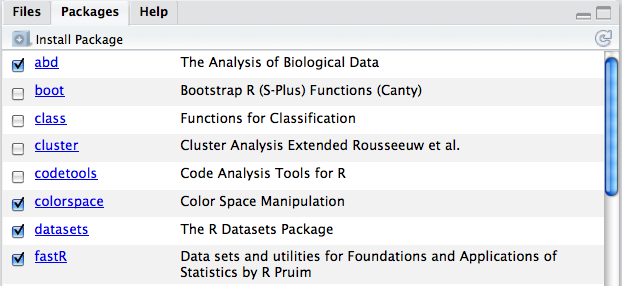
\includegraphics[width=.55\textwidth]{images/RStudio-packages}
\end{center}

%(A similar thing is true for the stand-alone versions of \R.)

Here are some packages we will use frequently:
\begin{itemize}
\item \verb!lattice!  (for graphics; this will always be installed in \R)
\item \verb!mosaic!  (for teaching statistics; this will need to be installed in \R\
from CRAN, see section \ref{sec:CRAN})
\item \verb!Hmisc!    (a package with some nice utilities; available on CRAN)
%\item \verb!vcd!      (a package for visualizing categorical data; available on CRAN)
%\item \verb!fastR!    (a package with some nice utilities; available on CRAN)
%\item \verb!abd!      (a package with some nice datasets; available on CRAN)
\end{itemize}
There are others that we use from time to time as well.  
%\verb!Hmisc!, \verb!vcd!, \verb!fastR!, \verb!abd!, and \verb!mosaic! 
\authNote{R': I think we can reduce to \verb!lattice! and \verb!mosaic!.  Possibly \verb!Hmisc!.
I'll remove dependencies on \verb!abd! as I go.}%
You should install \verb!Hmisc! and 
\verb!mosaic! the first time you use \R.
Once a package is installed, it is available to be loaded in the current or any future session.
You can install these packages 
by clicking on the ``Install Package" button in \RStudio\ and following the directions
or by using the following command:

\begin{knitrout}
\definecolor{shadecolor}{rgb}{.97, .97, .97}{\color{fgcolor}\begin{kframe}
\begin{flushleft}
\ttfamily\noindent
\hlfunctioncall{install.packages}\hlkeyword{(}\hlstring{"{}Hmisc"{}}\hlkeyword{)}{\ }{\ }\hlcomment{\usebox{\hlnormalsizeboxhash}{\ }note{\ }the{\ }quotation{\ }marks}\hspace*{\fill}\\
\hlstd{}\hlfunctioncall{install.packages}\hlkeyword{(}\hlstring{"{}mosaic"{}}\hlkeyword{)}{\ }{\ }\hlcomment{\usebox{\hlnormalsizeboxhash}{\ }note{\ }the{\ }quotation{\ }marks}\mbox{}
\normalfont
\end{flushleft}
\end{kframe}}
\end{knitrout}


Once these are installed, you can load them by checking the box in the 
\tab{Packages} tab or by using \verb!require()! (or \verb!library()!)

\begin{knitrout}
\definecolor{shadecolor}{rgb}{.97, .97, .97}{\color{fgcolor}\begin{kframe}
\begin{flushleft}
\ttfamily\noindent
\hlfunctioncall{require}\hlkeyword{(}\hlsymbol{lattice}\hlkeyword{)}{\ }{\ }\hlcomment{\usebox{\hlnormalsizeboxhash}{\ }could{\ }also{\ }use{\ }library(lattice)}\hspace*{\fill}\\
\hlstd{}\hlfunctioncall{require}\hlkeyword{(}\hlsymbol{Hmisc}\hlkeyword{)}{\ }{\ }\hlcomment{\usebox{\hlnormalsizeboxhash}{\ }do{\ }this{\ }one{\ }before{\ }mosaic}\hspace*{\fill}\\
\hlstd{}\hlfunctioncall{require}\hlkeyword{(}\hlsymbol{mosaic}\hlkeyword{)}{\ }{\ }\hlcomment{\usebox{\hlnormalsizeboxhash}{\ }do{\ }this{\ }one{\ }after{\ }Hmisc}\mbox{}
\normalfont
\end{flushleft}
\end{kframe}}
\end{knitrout}


\authNote{Add bibliography entries for books associated with packages.}
\begin{problem}
Install and load the \verb!mosaic! package.
Make sure \verb!lattice! is also loaded (no need to install it, it is already installed).

Here are some other packages you may like to install as well.
\authNote{we need fewer packages in this chapter!}
\begin{itemize}
\item
\verb!Hmisc! (Frank Harrell's miscellaneous utilities),
\item
\verb!vcd! (visualizing categorical data),
\item
\verb!fastR! (\textit{Foundations and Applications of Statistics}), and 
\item
\verb!abd! (\textit{Analysis of Biological Data}).
\end{itemize}
\end{problem}


\section{Getting Help}

If something doesn't go quite right, or if you can't remember something, it's good to know
where to turn for help.  In addition to asking your friends and neighbors, you can use
the \R\ help system.

\subsection{?}

To get help on a specific function or data set, simply precede its name with a \verb!?!:

\begin{knitrout}
\definecolor{shadecolor}{rgb}{.97, .97, .97}{\color{fgcolor}\begin{kframe}
\begin{flushleft}
\ttfamily\noindent
\hlfunctioncall{\usebox{\hlnormalsizeboxbacktick}?\usebox{\hlnormalsizeboxbacktick}}\hlkeyword{(}\hlfunctioncall{col.whitebg}\hlkeyword{(}\hlkeyword{)}\hlkeyword{)}\mbox{}
\normalfont
\end{flushleft}
\end{kframe}}
\end{knitrout}

%This will give you the documentation for the object you are interested in.

\subsection{\texttt{apropos()}}
If you don't know the exact name of a function, you can give part of the name and 
\R\ will find all functions that match.  Quotation marks are mandatory here.

\begin{knitrout}
\definecolor{shadecolor}{rgb}{.97, .97, .97}{\color{fgcolor}\begin{kframe}
\begin{flushleft}
\ttfamily\noindent
\hlfunctioncall{apropos}\hlkeyword{(}\hlstring{"{}hist"{}}\hlkeyword{)}{\ }{\ }\hlcomment{\usebox{\hlnormalsizeboxhash}{\ }must{\ }include{\ }quotes.{\ }{\ }single{\ }or{\ }double.}\mbox{}
\normalfont
\end{flushleft}
\begin{verbatim}
 [1] "event.history"              "hist"                       "hist.data.frame"           
 [4] "hist.default"               "hist.FD"                    "hist.scott"                
 [7] "histbackback"               "histogram"                  "histogram"                 
[10] "history"                    "histSpike"                  "ldahist"                   
[13] "loadhistory"                "panel.histogram"            "panel.xhistogram"          
[16] "pmfhistogram"               "prepanel.default.histogram" "savehistory"               
[19] "truehist"                   "xhistogram"                
\end{verbatim}
\end{kframe}}
\end{knitrout}


\subsection{\texttt{??} and \texttt{help.search()}}
If that fails, you can do a broader search using \verb!??! or \verb!help.search()!, 
which will find matches not only in the names of functions and data sets, 
but also in the documentation for them.  Quotations marks are optional here.

% <<help2,eval=FALSE,results=hide,echo=TRUE>>=
% ??histogram                  # any of these will work
% ??"histogram"  
% ??'histogram'  
% help.search('histogram')
% @


\subsection{Examples and Demos}

Many functions and data sets in \R\ include example code demonstrating typical uses.
For example,
\begin{knitrout}
\definecolor{shadecolor}{rgb}{.97, .97, .97}{\color{fgcolor}\begin{kframe}
\begin{flushleft}
\ttfamily\noindent
\hlfunctioncall{example}\hlkeyword{(}\hlsymbol{histogram}\hlkeyword{)}\mbox{}
\normalfont
\end{flushleft}
\end{kframe}}
\end{knitrout}

will generate a number of example plots (and provide you with the commands used to create them).
Examples such as this are intended to help you learn how specific \R\ functions work.
\FoodForThought{Not all package authors are equally skilled at creating examples.  
Some of the examples are next to useless, others are excellent.}
These examples also appear at the end of the documentation for functions and data sets.

The \verb!mosaic! package (and some other packages as well) also includes demos.  
Demos are bits of \R\ code that can be executed using the \verb!demo()! command
with the name of the demo.

To see how demos work, give this a try:
\begin{knitrout}
\definecolor{shadecolor}{rgb}{.97, .97, .97}{\color{fgcolor}\begin{kframe}
\begin{flushleft}
\ttfamily\noindent
\hlfunctioncall{demo}\hlkeyword{(}\hlsymbol{histogram}\hlkeyword{)}\mbox{}
\normalfont
\end{flushleft}
\end{kframe}}
\end{knitrout}


Demos are intended to illustrate a concept, a method, or some such thing, and are 
independent of any particular function or data set.

You can get a list of available demos using

\begin{knitrout}
\definecolor{shadecolor}{rgb}{.97, .97, .97}{\color{fgcolor}\begin{kframe}
\begin{flushleft}
\ttfamily\noindent
\hlfunctioncall{demo}\hlkeyword{(}\hlkeyword{)}{\ }{\ }\hlcomment{\usebox{\hlnormalsizeboxhash}{\ }all{\ }demos}\hspace*{\fill}\\
\hlstd{}\hlfunctioncall{demo}\hlkeyword{(}\hlargument{package}{\ }\hlargument{=}{\ }\hlstring{"{}mosaic"{}}\hlkeyword{)}{\ }{\ }\hlcomment{\usebox{\hlnormalsizeboxhash}{\ }just{\ }demos{\ }from{\ }mosaic{\ }package}\mbox{}
\normalfont
\end{flushleft}
\end{kframe}}
\end{knitrout}



\section{Data}
\subsection{Data in Packages}
Many packages contain data sets.  You can see a list of all data sets in all loaded packages
using 

\begin{knitrout}
\definecolor{shadecolor}{rgb}{.97, .97, .97}{\color{fgcolor}\begin{kframe}
\begin{flushleft}
\ttfamily\noindent
\hlfunctioncall{data}\hlkeyword{(}\hlkeyword{)}\mbox{}
\normalfont
\end{flushleft}
\end{kframe}}
\end{knitrout}


Typically (provide the author of the package allowed for lazy loading of data) 
you can use data sets by simply typing their names.  But if you have already
used that name for something or need to refresh the data after making some changes you no longer
want, you can explicitly load the data using the \verb!data()! function with the name of the 
data set you want.

\begin{knitrout}
\definecolor{shadecolor}{rgb}{.97, .97, .97}{\color{fgcolor}\begin{kframe}
\begin{flushleft}
\ttfamily\noindent
\hlfunctioncall{data}\hlkeyword{(}\hlsymbol{iris}\hlkeyword{)}\mbox{}
\normalfont
\end{flushleft}
\end{kframe}}
\end{knitrout}


\subsection{Data Frames}

Data sets are usually stored in a special structure called a \term{data frame}.

\begin{boxedText}
Data frames have a 2-dimensional structure.  
\medskip
\begin{itemize}
\item 
Rows correspond to 
\term{observational units} (people, animals, plants, or other objects we
are collecting data about).
\item
Columns correspond to \term{variables} (measurements collected on each 
observational unit).
\end{itemize}
\end{boxedText}

We'll talk later about how to get your own data into \R.  For now we'll use 
some data that comes with \R\ and is all ready for you to use.
The \verb!iris! data frame contains 5 \term{variables} measured for each
of 150 iris plants (the observational units).  
The \verb!iris! data set is included with the default \R\ installation.  
(Technically, it is located in a package called \verb!datasets!  which is always available.)

There are several ways we can get some idea about what is in the \verb!iris! data frame.

\begin{knitrout}
\definecolor{shadecolor}{rgb}{.97, .97, .97}{\color{fgcolor}\begin{kframe}
\begin{flushleft}
\ttfamily\noindent
\hlfunctioncall{str}\hlkeyword{(}\hlsymbol{iris}\hlkeyword{)}\mbox{}
\normalfont
\end{flushleft}
\begin{verbatim}
'data.frame':	150 obs. of  5 variables:
 $ Sepal.Length: num  5.1 4.9 4.7 4.6 5 5.4 4.6 5 4.4 4.9 ...
 $ Sepal.Width : num  3.5 3 3.2 3.1 3.6 3.9 3.4 3.4 2.9 3.1 ...
 $ Petal.Length: num  1.4 1.4 1.3 1.5 1.4 1.7 1.4 1.5 1.4 1.5 ...
 $ Petal.Width : num  0.2 0.2 0.2 0.2 0.2 0.4 0.3 0.2 0.2 0.1 ...
 $ Species     : Factor w/ 3 levels "setosa","versicolor",..: 1 1 1 1 1 1 1 1 1 1 ...
\end{verbatim}
\end{kframe}}
\end{knitrout}


\begin{knitrout}
\definecolor{shadecolor}{rgb}{.97, .97, .97}{\color{fgcolor}\begin{kframe}
\begin{flushleft}
\ttfamily\noindent
\hlfunctioncall{summary}\hlkeyword{(}\hlsymbol{iris}\hlkeyword{)}\mbox{}
\normalfont
\end{flushleft}
\begin{verbatim}
  Sepal.Length   Sepal.Width    Petal.Length   Petal.Width        Species  
 Min.   :4.30   Min.   :2.00   Min.   :1.00   Min.   :0.1   setosa    :50  
 1st Qu.:5.10   1st Qu.:2.80   1st Qu.:1.60   1st Qu.:0.3   versicolor:50  
 Median :5.80   Median :3.00   Median :4.35   Median :1.3   virginica :50  
 Mean   :5.84   Mean   :3.06   Mean   :3.76   Mean   :1.2                  
 3rd Qu.:6.40   3rd Qu.:3.30   3rd Qu.:5.10   3rd Qu.:1.8                  
 Max.   :7.90   Max.   :4.40   Max.   :6.90   Max.   :2.5                  
\end{verbatim}
\end{kframe}}
\end{knitrout}


\begin{knitrout}
\definecolor{shadecolor}{rgb}{.97, .97, .97}{\color{fgcolor}\begin{kframe}
\begin{flushleft}
\ttfamily\noindent
\hlfunctioncall{head}\hlkeyword{(}\hlsymbol{iris}\hlkeyword{)}\mbox{}
\normalfont
\end{flushleft}
\begin{verbatim}
  Sepal.Length Sepal.Width Petal.Length Petal.Width Species
1          5.1         3.5          1.4         0.2  setosa
2          4.9         3.0          1.4         0.2  setosa
3          4.7         3.2          1.3         0.2  setosa
4          4.6         3.1          1.5         0.2  setosa
5          5.0         3.6          1.4         0.2  setosa
6          5.4         3.9          1.7         0.4  setosa
\end{verbatim}
\end{kframe}}
\end{knitrout}

In interactive mode, you can also try
\begin{knitrout}
\definecolor{shadecolor}{rgb}{.97, .97, .97}{\color{fgcolor}\begin{kframe}
\begin{flushleft}
\ttfamily\noindent
\hlfunctioncall{View}\hlkeyword{(}\hlsymbol{iris}\hlkeyword{)}\mbox{}
\normalfont
\end{flushleft}
\end{kframe}}
\end{knitrout}

to see the data or 
\begin{knitrout}
\definecolor{shadecolor}{rgb}{.97, .97, .97}{\color{fgcolor}\begin{kframe}
\begin{flushleft}
\ttfamily\noindent
\hlfunctioncall{\usebox{\hlnormalsizeboxbacktick}?\usebox{\hlnormalsizeboxbacktick}}\hlkeyword{(}\hlsymbol{iris}\hlkeyword{)}\mbox{}
\normalfont
\end{flushleft}
\end{kframe}}
\end{knitrout}

to get the documentation about for the data set.

%\subsection{Getting at the Variables}
Access to an individual variable in a data frame uses the \verb!$! operator in
the following syntax:

\begin{knitrout}
\definecolor{shadecolor}{rgb}{.97, .97, .97}{\color{fgcolor}\begin{kframe}
\begin{flushleft}
\ttfamily\noindent
\hlsymbol{dataframe}\hlkeyword{\usebox{\hlnormalsizeboxdollar}}\hlsymbol{variable}\mbox{}
\normalfont
\end{flushleft}
\end{kframe}}
\end{knitrout}

or 
\begin{knitrout}
\definecolor{shadecolor}{rgb}{.97, .97, .97}{\color{fgcolor}\begin{kframe}
\begin{flushleft}
\ttfamily\noindent
\hlfunctioncall{with}\hlkeyword{(}\hlsymbol{dataframe}\hlkeyword{,}{\ }\hlsymbol{variable}\hlkeyword{)}\mbox{}
\normalfont
\end{flushleft}
\end{kframe}}
\end{knitrout}


For example, either of 

\begin{knitrout}
\definecolor{shadecolor}{rgb}{.97, .97, .97}{\color{fgcolor}\begin{kframe}
\begin{flushleft}
\ttfamily\noindent
\hlsymbol{iris}\hlkeyword{\usebox{\hlnormalsizeboxdollar}}\hlsymbol{Sepal.Length}\mbox{}
\normalfont
\end{flushleft}
\end{kframe}}
\end{knitrout}

or 
\begin{knitrout}
\definecolor{shadecolor}{rgb}{.97, .97, .97}{\color{fgcolor}\begin{kframe}
\begin{flushleft}
\ttfamily\noindent
\hlfunctioncall{with}\hlkeyword{(}\hlsymbol{iris}\hlkeyword{,}{\ }\hlsymbol{Sepal.Length}\hlkeyword{)}\mbox{}
\normalfont
\end{flushleft}
\end{kframe}}
\end{knitrout}

shows the contents of the \verb!Sepal.Length! variable in the following format.
\begin{knitrout}
\definecolor{shadecolor}{rgb}{.97, .97, .97}{\color{fgcolor}\begin{kframe}
\begin{verbatim}
  [1] 5.1 4.9 4.7 4.6 5.0 5.4 4.6 5.0 4.4 4.9 5.4 4.8 4.8 4.3 5.8 5.7 5.4 5.1 5.7 5.1 5.4 5.1 4.6
 [24] 5.1 4.8 5.0 5.0 5.2 5.2 4.7 4.8 5.4 5.2 5.5 4.9 5.0 5.5 4.9 4.4 5.1 5.0 4.5 4.4 5.0 5.1 4.8
 [47] 5.1 4.6 5.3 5.0 7.0 6.4 6.9 5.5 6.5 5.7 6.3 4.9 6.6 5.2 5.0 5.9 6.0 6.1 5.6 6.7 5.6 5.8 6.2
 [70] 5.6 5.9 6.1 6.3 6.1 6.4 6.6 6.8 6.7 6.0 5.7 5.5 5.5 5.8 6.0 5.4 6.0 6.7 6.3 5.6 5.5 5.5 6.1
 [93] 5.8 5.0 5.6 5.7 5.7 6.2 5.1 5.7 6.3 5.8 7.1 6.3 6.5 7.6 4.9 7.3 6.7 7.2 6.5 6.4 6.8 5.7 5.8
[116] 6.4 6.5 7.7 7.7 6.0 6.9 5.6 7.7 6.3 6.7 7.2 6.2 6.1 6.4 7.2 7.4 7.9 6.4 6.3 6.1 7.7 6.3 6.4
[139] 6.0 6.9 6.7 6.9 5.8 6.8 6.7 6.7 6.3 6.5 6.2 5.9
\end{verbatim}
\end{kframe}}
\end{knitrout}


But this isn't very useful for a large data set.  
We would prefer to compute numerical or graphical summaries.  We'll do that shortly.

The \verb!attach()! function in R can be used to make objects within dataframes
accessible in R with fewer keystrokes, but we strongly discourage its use, as
it often leads to name conflicts.  
\Caution{Avoid the use of \function{attach()}.}
The Google R Style Guide
(\url{http://google-styleguide.googlecode.com/svn/trunk/google-r-style.html})
echoes this advice, stating that \emph{The possibilities for creating errors
when using attach are numerous. Avoid it.} 
It is far better to directly access
variables using the \verb!\$! syntax or to use the \function{with()} function.

\subsection{Using Your Own Data}
\Rstudio\ will help you import your own data.  To do so use the ``Import Dataset" 
button in the \tab{Workspace} tab.  You can load data from text files, from the web, or from
google spreadsheets.   

%\subsubsection*{From Google Spreadsheets}

\textbf{From Google.}
The easiest of these is the Google spreadsheets option: Just click, select
your spreadsheet, choose a name, and you're done.

%\subsubsection*{From Excel}
\textbf{From Excel},
you need to follow a 3-step process:
\begin{enumerate}
\item
Save your Excel worksheet as a csv (comma separated value) file.
\item
Upload (in the \tab{Files} tab) your csv file to the server, where you can create folders and store
files in your personal account.  
(To share things with others: Put the files in your Public folder.  
Read the\texttt{AboutPublic.txt} file in that folder for directions.)
\item
Now import ``from a text file'' in the \tab{Workspace} tab.
\end{enumerate}

In either case, be sure to do the following:
\begin{itemize}
\item Choose good variables names.
\item Put your variables names in the first row.
\item Use each subsequent row for one observational unit.
\item Give the resulting data frame a good name.
\end{itemize}
\authNoted{I moved Danny's Simple Relational Database suggestion
to \ref{sec:manipulatingData}.
I don't think I would use a grade/courses example for students nor that
I would introduce \function{merge()} \emph{et al} to newbies right away.
My goal was to have this appendix look like something that I would give
to students as is in the first week.
In any case, I agree that we should have a section on this somewhere.
[RJP]
}%

If you are not using \RStudio, you can read files using
\function{read.csv()} or \function{read.table()} (for white space delimited files).
The \function{mosaic} package includes a function called \function{read.file()} that uses 
slightly different default settings and infers whether it should use \function{read.csv()},
\function{read.table()}, or \function{load()} based on the file name.  
\DiggingDeeper[\centerline{\function{load()}}]{\function{load()} is used
for opening files that store \R\ objects in `native' format.}

Each of these functions 
also accepts a URL in place of a file name, which provides an easy way to distribute data
via the Internet:
\begin{knitrout}
\definecolor{shadecolor}{rgb}{.97, .97, .97}{\color{fgcolor}\begin{kframe}
\begin{flushleft}
\ttfamily\noindent
\hlsymbol{births}{\ }\hlassignement{\usebox{\hlnormalsizeboxlessthan}-}{\ }\hlfunctioncall{read.table}\hlkeyword{(}\hlstring{"{}http://www.calvin.edu/\urltilda{}rpruim/data/births.txt"{}}\hlkeyword{,}\hspace*{\fill}\\
\hlstd{}{\ }{\ }{\ }{\ }\hlargument{header}{\ }\hlargument{=}{\ }\hlnumber{TRUE}\hlkeyword{)}\hspace*{\fill}\\
\hlstd{}\hlfunctioncall{head}\hlkeyword{(}\hlsymbol{births}\hlkeyword{)}{\ }{\ }\hlcomment{\usebox{\hlnormalsizeboxhash}{\ }number{\ }of{\ }live{\ }births{\ }in{\ }the{\ }US{\ }each{\ }day{\ }of{\ }1978.}\mbox{}
\normalfont
\end{flushleft}
\begin{verbatim}
    date births datenum dayofyear
1 1/1/78   7701    6575         1
2 1/2/78   7527    6576         2
3 1/3/78   8825    6577         3
4 1/4/78   8859    6578         4
5 1/5/78   9043    6579         5
6 1/6/78   9208    6580         6
\end{verbatim}
\end{kframe}}
\end{knitrout}

The \pkg{mosaic} package provides \function{read.file()} which attempts to infer
the file type from its extension and then applies 
\function{read.csv()}, \function{read.table()}, or \function{load()}.
\begin{knitrout}
\definecolor{shadecolor}{rgb}{.97, .97, .97}{\color{fgcolor}\begin{kframe}
\begin{flushleft}
\ttfamily\noindent
\hlsymbol{births}{\ }\hlassignement{\usebox{\hlnormalsizeboxlessthan}-}{\ }\hlfunctioncall{read.file}\hlkeyword{(}\hlstring{"{}http://www.calvin.edu/\urltilda{}rpruim/data/births.txt"{}}\hlkeyword{)}\mbox{}
\normalfont
\end{flushleft}
\end{kframe}}
\end{knitrout}

It also sets a number of defaults, including \option{header=TRUE}.

\begin{problem}
Enter the following small data set in an Excel or Google spreadsheet and import the 
data into \Rstudio.

\begin{center}
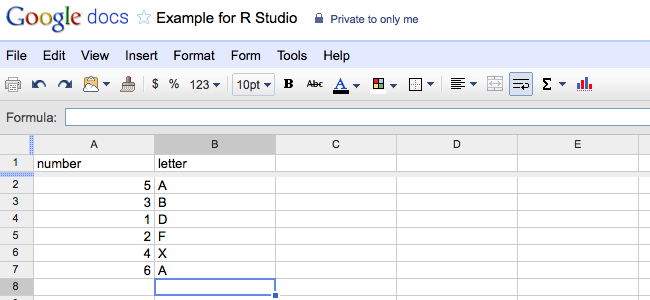
\includegraphics[width=.5\textwidth]{images/GoogleSpreadsheet}
\end{center}

You can import directly from Google.  From Excel, save the file as a csv and
import that (as a text file) into \Rstudio.  Name the data frame \texttt{JunkData}.
\end{problem}

\subsection{Putting Data Into a Package}

It is not that difficult to take a collection of csv files (a format available for many books)
and put them all into a package.
The \verb!abd! package contains data sets from \textit{The Analysis of Biological Data}, for example.  
Kevin Middleton and Randall Pruim contacted the authors and obtained permission to 
build and disseminate this package.

The \verb!abdData()! function in \verb!abd! makes it easy to map examples and exercises in that book to 
data frame names in the \verb!abd! package.

\begin{knitrout}
\definecolor{shadecolor}{rgb}{.97, .97, .97}{\color{fgcolor}\begin{kframe}
\begin{flushleft}
\ttfamily\noindent
\hlfunctioncall{abdData}\hlkeyword{(}\hlstring{"{}human"{}}\hlkeyword{)}{\ }{\ }\hlcomment{\usebox{\hlnormalsizeboxhash}{\ }all{\ }data{\ }sets{\ }with{\ }\usebox{\hlnormalsizeboxsinglequote}human\usebox{\hlnormalsizeboxsinglequote}{\ }in{\ }the{\ }name}\mbox{}
\normalfont
\end{flushleft}
\begin{verbatim}
Error: could not find function "abdData"
\end{verbatim}
\end{kframe}}
\end{knitrout}


\begin{knitrout}
\definecolor{shadecolor}{rgb}{.97, .97, .97}{\color{fgcolor}\begin{kframe}
\begin{flushleft}
\ttfamily\noindent
\hlfunctioncall{abdData}\hlkeyword{(}\hlnumber{2}\hlkeyword{)}{\ }{\ }\hlcomment{\usebox{\hlnormalsizeboxhash}{\ }all{\ }data{\ }sets{\ }in{\ }chapter{\ }2}\mbox{}
\normalfont
\end{flushleft}
\begin{verbatim}
Error: could not find function "abdData"
\end{verbatim}
\end{kframe}}
\end{knitrout}


For information on how to create such packages, consult the \textit{Writing R Extensions} manual
on CRAN.

\section{Summarizing Data}

\subsection{A Few Numerical Summaries}
\R\ includes functions that compute a wide range of numerical and graphical summaries.  
Most of the numerical summaries already familiar to you have obvious names.  
Here are a few examples.  
%(If you don't know what some of these -- like IQR -- are, don't worry;
%we'll be discussing them soon.)

\begin{knitrout}
\definecolor{shadecolor}{rgb}{.97, .97, .97}{\color{fgcolor}\begin{kframe}
\begin{flushleft}
\ttfamily\noindent
\hlfunctioncall{with}\hlkeyword{(}\hlsymbol{iris}\hlkeyword{,}{\ }\hlfunctioncall{mean}\hlkeyword{(}\hlsymbol{Sepal.Length}\hlkeyword{)}\hlkeyword{)}{\ }{\ }\hlcomment{\usebox{\hlnormalsizeboxhash}{\ }or{\ }mean(iris\usebox{\hlnormalsizeboxdollar}Sepal.Length)}\mbox{}
\normalfont
\end{flushleft}
\begin{verbatim}
 mean 
5.843 
\end{verbatim}
\begin{flushleft}
\ttfamily\noindent
\hlfunctioncall{with}\hlkeyword{(}\hlsymbol{iris}\hlkeyword{,}{\ }\hlfunctioncall{median}\hlkeyword{(}\hlsymbol{Sepal.Length}\hlkeyword{)}\hlkeyword{)}{\ }{\ }\hlcomment{\usebox{\hlnormalsizeboxhash}{\ }or{\ }median(iris\usebox{\hlnormalsizeboxdollar}Sepal.Length)}\mbox{}
\normalfont
\end{flushleft}
\begin{verbatim}
median 
   5.8 
\end{verbatim}
\begin{flushleft}
\ttfamily\noindent
\hlfunctioncall{with}\hlkeyword{(}\hlsymbol{iris}\hlkeyword{,}{\ }\hlfunctioncall{sd}\hlkeyword{(}\hlsymbol{Sepal.Length}\hlkeyword{)}\hlkeyword{)}{\ }{\ }\hlcomment{\usebox{\hlnormalsizeboxhash}{\ }or{\ }sd(iris\usebox{\hlnormalsizeboxdollar}Sepal.Length)}\mbox{}
\normalfont
\end{flushleft}
\begin{verbatim}
    sd 
0.8281 
\end{verbatim}
\begin{flushleft}
\ttfamily\noindent
\hlfunctioncall{with}\hlkeyword{(}\hlsymbol{iris}\hlkeyword{,}{\ }\hlfunctioncall{quantile}\hlkeyword{(}\hlsymbol{Sepal.Length}\hlkeyword{)}\hlkeyword{)}{\ }{\ }\hlcomment{\usebox{\hlnormalsizeboxhash}{\ }or{\ }quantile(iris\usebox{\hlnormalsizeboxdollar}Sepal.Length)}\mbox{}
\normalfont
\end{flushleft}
\begin{verbatim}
  0%  25%  50%  75% 100% 
 4.3  5.1  5.8  6.4  7.9 
\end{verbatim}
\begin{flushleft}
\ttfamily\noindent
\hlfunctioncall{with}\hlkeyword{(}\hlsymbol{iris}\hlkeyword{,}{\ }\hlfunctioncall{IQR}\hlkeyword{(}\hlsymbol{Sepal.Length}\hlkeyword{)}\hlkeyword{)}{\ }{\ }\hlcomment{\usebox{\hlnormalsizeboxhash}{\ }or{\ }IQR(iris\usebox{\hlnormalsizeboxdollar}Sepal.Length)}\mbox{}
\normalfont
\end{flushleft}
\begin{verbatim}
[1] 1.3
\end{verbatim}
\begin{flushleft}
\ttfamily\noindent
\hlfunctioncall{IQR}\hlkeyword{(}\hlsymbol{iris}\hlkeyword{\usebox{\hlnormalsizeboxdollar}}\hlsymbol{Sepal.Length}\hlkeyword{)}\mbox{}
\normalfont
\end{flushleft}
\begin{verbatim}
[1] 1.3
\end{verbatim}
\end{kframe}}
\end{knitrout}


The \verb!favstats()! function in the \verb!mosaic! package computes several numerical 
summaries all at once.

\begin{knitrout}
\definecolor{shadecolor}{rgb}{.97, .97, .97}{\color{fgcolor}\begin{kframe}
\begin{flushleft}
\ttfamily\noindent
\hlfunctioncall{require}\hlkeyword{(}\hlsymbol{mosaic}\hlkeyword{)}{\ }{\ }\hlcomment{\usebox{\hlnormalsizeboxhash}{\ }if{\ }you{\ }haven\usebox{\hlnormalsizeboxsinglequote}t{\ }already{\ }loaded{\ }the{\ }mosaic{\ }package}\hspace*{\fill}\\
\hlstd{}\hlfunctioncall{favstats}\hlkeyword{(}\hlsymbol{iris}\hlkeyword{\usebox{\hlnormalsizeboxdollar}}\hlsymbol{Sepal.Length}\hlkeyword{)}\mbox{}
\normalfont
\end{flushleft}
\begin{verbatim}
    0%    25%    50%    75%   100%   mean     sd    var 
4.3000 5.1000 5.8000 6.4000 7.9000 5.8433 0.8281 0.6857 
\end{verbatim}
\end{kframe}}
\end{knitrout}


Here's something a little fancier.

\begin{knitrout}
\definecolor{shadecolor}{rgb}{.97, .97, .97}{\color{fgcolor}\begin{kframe}
\begin{flushleft}
\ttfamily\noindent
\hlfunctioncall{require}\hlkeyword{(}\hlsymbol{Hmisc}\hlkeyword{)}\hspace*{\fill}\\
\hlstd{}\hlfunctioncall{summary}\hlkeyword{(}\hlsymbol{Sepal.Length}{\ }\hlkeyword{\urltilda{}}{\ }\hlsymbol{Species}\hlkeyword{,}{\ }\hlargument{data}{\ }\hlargument{=}{\ }\hlsymbol{iris}\hlkeyword{,}{\ }\hlargument{fun}{\ }\hlargument{=}{\ }\hlsymbol{favstats}\hlkeyword{)}\mbox{}
\normalfont
\end{flushleft}
\begin{verbatim}
Sepal.Length    N=150

+-------+----------+---+---+-----+---+---+----+-----+------+------+
|       |          |N  |0% |25%  |50%|75%|100%|mean |sd    |var   |
+-------+----------+---+---+-----+---+---+----+-----+------+------+
|Species|setosa    | 50|4.3|4.800|5.0|5.2|5.8 |5.006|0.3525|0.1242|
|       |versicolor| 50|4.9|5.600|5.9|6.3|7.0 |5.936|0.5162|0.2664|
|       |virginica | 50|4.9|6.225|6.5|6.9|7.9 |6.588|0.6359|0.4043|
+-------+----------+---+---+-----+---+---+----+-----+------+------+
|Overall|          |150|4.3|5.100|5.8|6.4|7.9 |5.843|0.8281|0.6857|
+-------+----------+---+---+-----+---+---+----+-----+------+------+
\end{verbatim}
\end{kframe}}
\end{knitrout}

(Note: This requires installation of the \verb!Hmisc! package.)

\begin{problem}
What is the average (mean) \emph{width} of the sepals in the \verb!iris! data set?
\end{problem}

\begin{problem}
Determine the average (mean) sepal width for each of the three species in the \verb!iris! data set.
\end{problem}

\subsection{Lattice Graphics}

There are several ways to make graphs in \R.  One approach is a system called
\verb!lattice! graphics.  The first step for using \verb!lattice! is to
load the \verb!lattice! package using the check box in the \tab{Packages} tab or using
the following command:

\begin{knitrout}
\definecolor{shadecolor}{rgb}{.97, .97, .97}{\color{fgcolor}\begin{kframe}
\begin{flushleft}
\ttfamily\noindent
\hlfunctioncall{require}\hlkeyword{(}\hlsymbol{lattice}\hlkeyword{)}\mbox{}
\normalfont
\end{flushleft}
\end{kframe}}
\end{knitrout}

\verb!lattice! plots make use of a \term{formula interface}:

\begin{knitrout}
\definecolor{shadecolor}{rgb}{.97, .97, .97}{\color{fgcolor}\begin{kframe}
\begin{flushleft}
\ttfamily\noindent
\hlfunctioncall{plotname}\hlkeyword{(}\hlsymbol{y}{\ }\hlkeyword{\urltilda{}}{\ }\hlsymbol{x}{\ }\hlkeyword{|}{\ }\hlsymbol{z}\hlkeyword{,}{\ }\hlargument{data}{\ }\hlargument{=}{\ }\hlsymbol{dataname}\hlkeyword{,}{\ }\hlargument{groups}{\ }\hlargument{=}{\ }\hlsymbol{grouping\usebox{\hlnormalsizeboxunderscore}variable}\hlkeyword{,}\hspace*{\fill}\\
\hlstd{}{\ }{\ }{\ }{\ }\hlsymbol{...}\hlkeyword{)}\mbox{}
\normalfont
\end{flushleft}
\end{kframe}}
\end{knitrout}

\begin{itemize}
\item
Here are the names of several \verb!lattice! plots:
\begin{itemize}
\item \verb!dotPlot! (notice the capital P; \verb!dotplot()! does something different)
\footnote{\texttt{dotPlot()} is in the \texttt{mosaic} package and was created because \texttt{dotplot()} in
the \texttt{lattice} package makes something different from what we call a dot plot.}
\item \verb!histogram!  (for histograms)
\item \verb!bwplot!  (for boxplots)
\item \verb!xyplot!  (for scatter plots)
\item \verb!qqmath!  (for quantile-quantile plots)
\end{itemize}
\item
\verb!x! is the name of the variable that is plotted along the horizontal 
($x$) axis.
\item
\verb!y! is the name of the variable that is plotted along the vertical ($y$) 
axis.  (For some plots, this slot is empty because \R\ computes these values
from the values of \verb!x!.)
\item
\verb!z! is a conditioning variable used to split the plot into 
multiple subplots called \term{panels}.
\item
\verb!grouping_variable! is used to display different groups differently
(different colors or symbols, for example) within the same panel.
\item
\verb!...! There are many additional arguments to these functions that let you
control just how the plots look.  (But we'll focus on the basics for now.)
\end{itemize}

%\subsection*{Some Examples}

\subsection{Dot plots: \texttt{dotPlot()}}

A dot plot represents each value of a quantitative variable with a dot.  The values
are rounded a bit so that the dots line up neatly, and dots are stacked up into little
towers when the data values cluster near each other.

For a dot plot, the \verb!y! component of the formula is empty since we let \R\
calculate that for us.

\begin{knitrout}
\definecolor{shadecolor}{rgb}{.97, .97, .97}{\color{fgcolor}\begin{kframe}
\begin{flushleft}
\ttfamily\noindent
\hlcomment{\usebox{\hlnormalsizeboxhash}{\ }was{\ }dotPlot}\hspace*{\fill}\\
\hlstd{}\hlfunctioncall{histogram}\hlkeyword{(}\hlkeyword{\urltilda{}}\hlsymbol{Sepal.Length}\hlkeyword{,}{\ }\hlargument{data}{\ }\hlargument{=}{\ }\hlsymbol{iris}\hlkeyword{,}{\ }\hlargument{n}{\ }\hlargument{=}{\ }\hlnumber{20}\hlkeyword{)}{\ }{\ }\hlcomment{\usebox{\hlnormalsizeboxhash}{\ }n=20{\ }gives{\ }us{\ }approximately{\ }20{\ }towers}\mbox{}
\normalfont
\end{flushleft}


\centering{}\includegraphics{figures/fig-iris-dotPlot} 

\end{kframe}}
\end{knitrout}

We can use a conditional variable to give us separate dot plots for each species.

\begin{knitrout}
\definecolor{shadecolor}{rgb}{.97, .97, .97}{\color{fgcolor}\begin{kframe}
\begin{flushleft}
\ttfamily\noindent
\hlcomment{\usebox{\hlnormalsizeboxhash}{\ }was{\ }dotPlot}\hspace*{\fill}\\
\hlstd{}\hlfunctioncall{histogram}\hlkeyword{(}\hlkeyword{\urltilda{}}\hlsymbol{Sepal.Length}{\ }\hlkeyword{|}{\ }\hlsymbol{Species}\hlkeyword{,}{\ }\hlargument{data}{\ }\hlargument{=}{\ }\hlsymbol{iris}\hlkeyword{,}{\ }\hlargument{n}{\ }\hlargument{=}{\ }\hlnumber{20}\hlkeyword{)}\mbox{}
\normalfont
\end{flushleft}
\end{kframe}}
\end{knitrout}

\begin{knitrout}
\definecolor{shadecolor}{rgb}{.97, .97, .97}{\color{fgcolor}\begin{kframe}


\centering{}\includegraphics{figures/fig-iris-dotPlot-condB} 

\end{kframe}}
\end{knitrout}


\subsection{Histograms: \texttt{histogram()}}

Histograms are a lot like dot plots, but the towers of dots are replaced by a vertical bar.
Again the \verb!y! component of the formula is empty since we let \R\
compute the heights of the bars for us.
\begin{knitrout}
\definecolor{shadecolor}{rgb}{.97, .97, .97}{\color{fgcolor}\begin{kframe}
\begin{flushleft}
\ttfamily\noindent
\hlfunctioncall{histogram}\hlkeyword{(}\hlkeyword{\urltilda{}}\hlsymbol{Sepal.Length}\hlkeyword{,}{\ }\hlargument{data}{\ }\hlargument{=}{\ }\hlsymbol{iris}\hlkeyword{,}{\ }\hlargument{n}{\ }\hlargument{=}{\ }\hlnumber{20}\hlkeyword{)}{\ }{\ }\hlcomment{\usebox{\hlnormalsizeboxhash}{\ }n={\ }20{\ }gives{\ }approx.{\ }20{\ }bars}\mbox{}
\normalfont
\end{flushleft}


\centering{}\includegraphics{figures/fig-iris-histogram} 

\end{kframe}}
\end{knitrout}

We can use a conditional variable to give us separate histograms for each species.

\begin{knitrout}
\definecolor{shadecolor}{rgb}{.97, .97, .97}{\color{fgcolor}\begin{kframe}
\begin{flushleft}
\ttfamily\noindent
\hlfunctioncall{histogram}\hlkeyword{(}\hlkeyword{\urltilda{}}\hlsymbol{Sepal.Length}{\ }\hlkeyword{|}{\ }\hlsymbol{Species}\hlkeyword{,}{\ }\hlargument{data}{\ }\hlargument{=}{\ }\hlsymbol{iris}\hlkeyword{,}{\ }\hlargument{n}{\ }\hlargument{=}{\ }\hlnumber{20}\hlkeyword{)}\mbox{}
\normalfont
\end{flushleft}


\centering{}\includegraphics{figures/fig-iris-histogram-cond} 

\end{kframe}}
\end{knitrout}



In lattice lingo, the three subplots are called panels and the 
labels at the top are called strips.  (Strips can be placed on the left side if you 
prefer.)


\subsection{Boxplots:  \texttt{bwplot()}}

Boxplots are made pretty much the same way as histograms:
\begin{knitrout}
\definecolor{shadecolor}{rgb}{.97, .97, .97}{\color{fgcolor}\begin{kframe}
\begin{flushleft}
\ttfamily\noindent
\hlfunctioncall{bwplot}\hlkeyword{(}\hlkeyword{\urltilda{}}\hlsymbol{Sepal.Length}\hlkeyword{,}{\ }\hlargument{data}{\ }\hlargument{=}{\ }\hlsymbol{iris}\hlkeyword{)}\mbox{}
\normalfont
\end{flushleft}


\centering{}\includegraphics{figures/fig-iris-bwplot} 

\end{kframe}}
\end{knitrout}


We can use conditioning as we did for histograms:

\begin{knitrout}
\definecolor{shadecolor}{rgb}{.97, .97, .97}{\color{fgcolor}\begin{kframe}
\begin{flushleft}
\ttfamily\noindent
\hlfunctioncall{bwplot}\hlkeyword{(}\hlkeyword{\urltilda{}}\hlsymbol{Sepal.Length}{\ }\hlkeyword{|}{\ }\hlsymbol{Species}\hlkeyword{,}{\ }\hlargument{data}{\ }\hlargument{=}{\ }\hlsymbol{iris}\hlkeyword{)}\mbox{}
\normalfont
\end{flushleft}


\centering{}\includegraphics{figures/fig-iris-bwplot-cond} 

\end{kframe}}
\end{knitrout}


\vspace{-8mm}

But there are better ways to do this.
\begin{knitrout}
\definecolor{shadecolor}{rgb}{.97, .97, .97}{\color{fgcolor}\begin{kframe}
\begin{flushleft}
\ttfamily\noindent
\hlfunctioncall{bwplot}\hlkeyword{(}\hlsymbol{Sepal.Length}{\ }\hlkeyword{\urltilda{}}{\ }\hlsymbol{Species}\hlkeyword{,}{\ }\hlargument{data}{\ }\hlargument{=}{\ }\hlsymbol{iris}\hlkeyword{)}\mbox{}
\normalfont
\end{flushleft}


\centering{}\includegraphics{figures/fig-iris-bwplot-2d} 

\end{kframe}}
\end{knitrout}

This is improved, but the species names run into each other.
We could fix that run-together text by using abbreviated names or rotating the
labels 45 or 90 degrees.  Instead of those solutions, we can also just reverse the roles
of the horizontal and vertical axes.
\begin{knitrout}
\definecolor{shadecolor}{rgb}{.97, .97, .97}{\color{fgcolor}\begin{kframe}
\begin{flushleft}
\ttfamily\noindent
\hlfunctioncall{bwplot}\hlkeyword{(}\hlsymbol{Species}{\ }\hlkeyword{\urltilda{}}{\ }\hlsymbol{Sepal.Length}\hlkeyword{,}{\ }\hlargument{data}{\ }\hlargument{=}{\ }\hlsymbol{iris}\hlkeyword{)}\mbox{}
\normalfont
\end{flushleft}


\centering{}\includegraphics{figures/fig-iris-bwplot-2dh} 

\end{kframe}}
\end{knitrout}


\vspace{-12mm}

%\pagebreak

\subsection{Scatterplots: \texttt{xyplot()}}

Scatterplots are made with \verb!xyplot()!.  The formula interface is very natural for this.  
Just remember that the ``$y$ variable'' comes first.  (Its label is also farther left on 
the plot, if that helps you remember.)
\begin{knitrout}
\definecolor{shadecolor}{rgb}{.97, .97, .97}{\color{fgcolor}\begin{kframe}
\begin{flushleft}
\ttfamily\noindent
\hlfunctioncall{xyplot}\hlkeyword{(}\hlsymbol{Sepal.Length}{\ }\hlkeyword{\urltilda{}}{\ }\hlsymbol{Sepal.Width}\hlkeyword{,}{\ }\hlargument{data}{\ }\hlargument{=}{\ }\hlsymbol{iris}\hlkeyword{)}\mbox{}
\normalfont
\end{flushleft}


\centering{}\includegraphics{figures/fig-iris-xyplot} 

\end{kframe}}
\end{knitrout}


Again, we can use conditioning to make a panel for each species.
\begin{knitrout}
\definecolor{shadecolor}{rgb}{.97, .97, .97}{\color{fgcolor}\begin{kframe}
\begin{flushleft}
\ttfamily\noindent
\hlfunctioncall{xyplot}\hlkeyword{(}\hlsymbol{Sepal.Length}{\ }\hlkeyword{\urltilda{}}{\ }\hlsymbol{Sepal.Width}{\ }\hlkeyword{|}{\ }\hlsymbol{Species}\hlkeyword{,}{\ }\hlargument{data}{\ }\hlargument{=}{\ }\hlsymbol{iris}\hlkeyword{)}\mbox{}
\normalfont
\end{flushleft}


\centering{}\includegraphics{figures/fig-iris-xyplot-cond} 

\end{kframe}}
\end{knitrout}



Even better (for this example), we can use the \verb!groups! argument to indicate the different species using
different symbols on the same panel.
\begin{knitrout}
\definecolor{shadecolor}{rgb}{.97, .97, .97}{\color{fgcolor}\begin{kframe}
\begin{flushleft}
\ttfamily\noindent
\hlfunctioncall{xyplot}\hlkeyword{(}\hlsymbol{Sepal.Length}{\ }\hlkeyword{\urltilda{}}{\ }\hlsymbol{Sepal.Width}\hlkeyword{,}{\ }\hlargument{groups}{\ }\hlargument{=}{\ }\hlsymbol{Species}\hlkeyword{,}{\ }\hlargument{data}{\ }\hlargument{=}{\ }\hlsymbol{iris}\hlkeyword{)}\mbox{}
\normalfont
\end{flushleft}


\centering{}\includegraphics{figures/fig-iris-xyplot-groups} 

\end{kframe}}
\end{knitrout}


\subsection{Saving Your Plots}

There are several ways to save plots, but the easiest is probably the following:
\begin{enumerate}
\item
In the \tab{Plots} tab, click the ``Export'' button.
\item
Copy the image to the clipboard using right click.
\item
Go to your Word document and paste in the image.
\item
Resize or reposition your image in Word as needed.
\end{enumerate}

\subsection{A Few Bells and Whistles}
There are lots of arguments that control how these plots look.  Here are just a few examples.

\subsubsection{auto.key}
It would be useful to have a legend for the previous plot.   \verb!auto.key=TRUE! 
turns on a simple legend.  (There are ways to have more control, if you need it.)
\begin{knitrout}
\definecolor{shadecolor}{rgb}{.97, .97, .97}{\color{fgcolor}\begin{kframe}
\begin{flushleft}
\ttfamily\noindent
\hlfunctioncall{xyplot}\hlkeyword{(}\hlsymbol{Sepal.Length}{\ }\hlkeyword{\urltilda{}}{\ }\hlsymbol{Sepal.Width}\hlkeyword{,}{\ }\hlargument{groups}{\ }\hlargument{=}{\ }\hlsymbol{Species}\hlkeyword{,}{\ }\hlargument{data}{\ }\hlargument{=}{\ }\hlsymbol{iris}\hlkeyword{,}\hspace*{\fill}\\
\hlstd{}{\ }{\ }{\ }{\ }\hlargument{auto.key}{\ }\hlargument{=}{\ }\hlnumber{TRUE}\hlkeyword{)}\mbox{}
\normalfont
\end{flushleft}


\centering{}\includegraphics{figures/fig-iris-xyplot-key} 

\end{kframe}}
\end{knitrout}


\subsubsection{alpha, cex}
Sometimes it is nice to have elements of a plot be partly transparent.  When such
elements overlap, they get darker, showing us where data are ``piling up."
Setting the \verb!alpha! argument to a value between 0 and 1 controls the degree 
of transparency: 1 is completely opaque, 0 is invisible.
The \verb!cex! argument controls ``character expansion" and can be used to make the 
plotting ``characters" larger or smaller by specifying the scaling ratio.
\begin{knitrout}
\definecolor{shadecolor}{rgb}{.97, .97, .97}{\color{fgcolor}\begin{kframe}
\begin{flushleft}
\ttfamily\noindent
\hlfunctioncall{xyplot}\hlkeyword{(}\hlsymbol{Sepal.Length}{\ }\hlkeyword{\urltilda{}}{\ }\hlsymbol{Sepal.Width}\hlkeyword{,}{\ }\hlargument{groups}{\ }\hlargument{=}{\ }\hlsymbol{Species}\hlkeyword{,}{\ }\hlargument{data}{\ }\hlargument{=}{\ }\hlsymbol{iris}\hlkeyword{,}\hspace*{\fill}\\
\hlstd{}{\ }{\ }{\ }{\ }\hlargument{auto.key}{\ }\hlargument{=}{\ }\hlfunctioncall{list}\hlkeyword{(}\hlargument{columns}{\ }\hlargument{=}{\ }\hlnumber{3}\hlkeyword{)}\hlkeyword{,}{\ }\hlargument{alpha}{\ }\hlargument{=}{\ }\hlnumber{0.5}\hlkeyword{,}{\ }\hlargument{cex}{\ }\hlargument{=}{\ }\hlnumber{1.3}\hlkeyword{)}\mbox{}
\normalfont
\end{flushleft}


\centering{}\includegraphics{figures/fig-iris-xyplot-alpha} 

\end{kframe}}
\end{knitrout}


\vspace{-8mm}
\subsubsection*{main, sub, xlab, ylab}

You can add a title or subtitle, or change the default labels of the axes.
\begin{knitrout}
\definecolor{shadecolor}{rgb}{.97, .97, .97}{\color{fgcolor}\begin{kframe}
\begin{flushleft}
\ttfamily\noindent
\hlfunctioncall{xyplot}\hlkeyword{(}\hlsymbol{Sepal.Length}{\ }\hlkeyword{\urltilda{}}{\ }\hlsymbol{Sepal.Width}\hlkeyword{,}{\ }\hlargument{groups}{\ }\hlargument{=}{\ }\hlsymbol{Species}\hlkeyword{,}{\ }\hlargument{data}{\ }\hlargument{=}{\ }\hlsymbol{iris}\hlkeyword{,}\hspace*{\fill}\\
\hlstd{}{\ }{\ }{\ }{\ }\hlargument{main}{\ }\hlargument{=}{\ }\hlstring{"{}Some{\ }Iris{\ }Data"{}}\hlkeyword{,}{\ }\hlargument{sub}{\ }\hlargument{=}{\ }\hlstring{"{}(R.{\ }A.{\ }Fisher{\ }analysized{\ }this{\ }data{\ }in{\ }1936)"{}}\hlkeyword{,}\hspace*{\fill}\\
\hlstd{}{\ }{\ }{\ }{\ }\hlargument{xlab}{\ }\hlargument{=}{\ }\hlstring{"{}sepal{\ }width{\ }(cm)"{}}\hlkeyword{,}{\ }\hlargument{ylab}{\ }\hlargument{=}{\ }\hlstring{"{}sepal{\ }length{\ }(cm)"{}}\hlkeyword{,}{\ }\hlargument{alpha}{\ }\hlargument{=}{\ }\hlnumber{0.5}\hlkeyword{,}{\ }\hlargument{auto.key}{\ }\hlargument{=}{\ }\hlfunctioncall{list}\hlkeyword{(}\hlargument{columns}{\ }\hlargument{=}{\ }\hlnumber{3}\hlkeyword{)}\hlkeyword{)}\mbox{}
\normalfont
\end{flushleft}


\centering{}\includegraphics{figures/fig-iris-xyplot-text} 

\end{kframe}}
\end{knitrout}


\subsubsection{trellis.par.set()}
Default settings for lattice graphics are set using 
\verb!trellis.par.set()!.
Don't like the default font sizes?  You can change to a 7 point (base) font using

\begin{knitrout}
\definecolor{shadecolor}{rgb}{.97, .97, .97}{\color{fgcolor}\begin{kframe}
\begin{flushleft}
\ttfamily\noindent
\hlfunctioncall{trellis.par.set}\hlkeyword{(}\hlargument{fontsize}{\ }\hlargument{=}{\ }\hlfunctioncall{list}\hlkeyword{(}\hlargument{text}{\ }\hlargument{=}{\ }\hlnumber{7}\hlkeyword{)}\hlkeyword{)}{\ }{\ }\hlcomment{\usebox{\hlnormalsizeboxhash}{\ }base{\ }size{\ }for{\ }text{\ }is{\ }7{\ }point}\mbox{}
\normalfont
\end{flushleft}
\end{kframe}}
\end{knitrout}



Nearly every feature of a lattice plot can be controlled: fonts, colors,
symbols, line thicknesses, colors, etc.
Rather than describe them all here, we'll mention only that groups of these settings 
can be collected into a theme.  \verb!show.settings()! will show you what the theme looks like.

\begin{knitrout}
\definecolor{shadecolor}{rgb}{.97, .97, .97}{\color{fgcolor}\begin{kframe}
\begin{flushleft}
\ttfamily\noindent
\hlfunctioncall{trellis.par.set}\hlkeyword{(}\hlargument{theme}{\ }\hlargument{=}{\ }\hlfunctioncall{col.whitebg}\hlkeyword{(}\hlkeyword{)}\hlkeyword{)}{\ }{\ }\hlcomment{\usebox{\hlnormalsizeboxhash}{\ }a{\ }theme{\ }in{\ }the{\ }lattice{\ }package}\hspace*{\fill}\\
\hlstd{}\hlfunctioncall{show.settings}\hlkeyword{(}\hlkeyword{)}\mbox{}
\normalfont
\end{flushleft}


\centering{}\includegraphics{figures/fig-themes-whitbg} 

\end{kframe}}
\end{knitrout}


\begin{knitrout}
\definecolor{shadecolor}{rgb}{.97, .97, .97}{\color{fgcolor}\begin{kframe}
\begin{flushleft}
\ttfamily\noindent
\hlfunctioncall{trellis.par.set}\hlkeyword{(}\hlargument{theme}{\ }\hlargument{=}{\ }\hlfunctioncall{col.abd}\hlkeyword{(}\hlkeyword{)}\hlkeyword{)}{\ }{\ }\hlcomment{\usebox{\hlnormalsizeboxhash}{\ }a{\ }theme{\ }in{\ }the{\ }abd{\ }package}\mbox{}
\normalfont
\end{flushleft}
\begin{verbatim}
Error: could not find function "col.abd"
\end{verbatim}
\begin{flushleft}
\ttfamily\noindent
\hlfunctioncall{show.settings}\hlkeyword{(}\hlkeyword{)}\mbox{}
\normalfont
\end{flushleft}


\centering{}\includegraphics{figures/fig-themes-abd} 

\end{kframe}}
\end{knitrout}


\begin{knitrout}
\definecolor{shadecolor}{rgb}{.97, .97, .97}{\color{fgcolor}\begin{kframe}
\begin{flushleft}
\ttfamily\noindent
\hlfunctioncall{trellis.par.set}\hlkeyword{(}\hlargument{theme}{\ }\hlargument{=}{\ }\hlfunctioncall{col.mosaic}\hlkeyword{(}\hlkeyword{)}\hlkeyword{)}{\ }{\ }\hlcomment{\usebox{\hlnormalsizeboxhash}{\ }a{\ }theme{\ }in{\ }the{\ }mosaic{\ }package}\hspace*{\fill}\\
\hlstd{}\hlfunctioncall{show.settings}\hlkeyword{(}\hlkeyword{)}\mbox{}
\normalfont
\end{flushleft}


\centering{}\includegraphics{figures/fig-themes-mosaic} 

\end{kframe}}
\end{knitrout}

\SuggestionBox{Do you have a great eye for colors?  Help us design other 
lattice themes.}%

\DiggingDeeper{The \pkg{RColorBrewer} package provides several
palettes of colors that are highly distinguishable and aesthetically pleasing.}%
\begin{knitrout}
\definecolor{shadecolor}{rgb}{.97, .97, .97}{\color{fgcolor}\begin{kframe}
\begin{flushleft}
\ttfamily\noindent
\hlfunctioncall{trellis.par.set}\hlkeyword{(}\hlargument{theme}{\ }\hlargument{=}{\ }\hlfunctioncall{col.mosaic}\hlkeyword{(}\hlargument{bw}{\ }\hlargument{=}{\ }\hlnumber{TRUE}\hlkeyword{)}\hlkeyword{)}{\ }{\ }\hlcomment{\usebox{\hlnormalsizeboxhash}{\ }black{\ }and{\ }white{\ }version{\ }of{\ }previous{\ }theme}\hspace*{\fill}\\
\hlstd{}\hlfunctioncall{show.settings}\hlkeyword{(}\hlkeyword{)}\mbox{}
\normalfont
\end{flushleft}


\centering{}\includegraphics{figures/fig-themes-mosaicbw} 

\end{kframe}}
\end{knitrout}


\begin{knitrout}
\definecolor{shadecolor}{rgb}{.97, .97, .97}{\color{fgcolor}\begin{kframe}
\begin{flushleft}
\ttfamily\noindent
\hlfunctioncall{trellis.par.set}\hlkeyword{(}\hlargument{theme}{\ }\hlargument{=}{\ }\hlfunctioncall{col.mosaic}\hlkeyword{(}\hlkeyword{)}\hlkeyword{)}{\ }{\ }\hlcomment{\usebox{\hlnormalsizeboxhash}{\ }back{\ }to{\ }the{\ }mosaic{\ }theme}\hspace*{\fill}\\
\hlstd{}\hlfunctioncall{trellis.par.set}\hlkeyword{(}\hlargument{fontsize}{\ }\hlargument{=}{\ }\hlfunctioncall{list}\hlkeyword{(}\hlargument{text}{\ }\hlargument{=}{\ }\hlnumber{9}\hlkeyword{)}\hlkeyword{)}{\ }{\ }\hlcomment{\usebox{\hlnormalsizeboxhash}{\ }and{\ }back{\ }to{\ }a{\ }larger{\ }font}\mbox{}
\normalfont
\end{flushleft}
\end{kframe}}
\end{knitrout}


\begin{problem}
The \verb!Jordan8687! data set (in the \verb!fastR! package) contains the number 
of points Michael Jordan scored in each game of the 1986--87 season.  
\begin{enumerate}
\item
Make a histogram of this data.  Add an appropriate title.
\item
How would you describe the shape of the distribution?
\item
In approximately what percentage of his games, did Michael Jordan score less than 20 points?
More than 50?
(You may want to add \verb!breaks=seq(0,70,by=5)! to your command to neaten up
the bins.)
\end{enumerate}
\end{problem}

\begin{problem}
Cuckoos lay their eggs in the nests of other birds.  Is the size of cuckoo eggs different
in different host species nests?  The \verb!cuckoo! data set (in \verb!fastR!)
contains data from a study attempting to answer this question.
\begin{enumerate}
\item
When were these data collected?  (Use \verb!?cuckoo! to get information about the data set.)
\item
What are the units on the length measurements?
\item
Make side-by-side boxplots of the length of the eggs by species.
\item
Calculate the mean length of the eggs for each host species.
\item
What do you think?  Does it look like the size is differs among the different host
species?  Refer to your \R\ output as you answer this question.
(We'll learn formal methods to investigate this later in the semester.)
\end{enumerate}
\vspace{-5mm}
\end{problem}

%\subsection{Bar Charts and Pie Charts}
\subsection{Tabulating Categorical Data}
The Current Population Survey (CPS) is used to supplement census information
between census years. These \dfn{CPS} data frame consist of a random sample of persons from the
CPS, with information on wages and other characteristics of the workers,
including sex, number of years of education, years of work experience,
occupational status, region of residence and union membership.


\begin{knitrout}
\definecolor{shadecolor}{rgb}{.97, .97, .97}{\color{fgcolor}\begin{kframe}
\begin{flushleft}
\ttfamily\noindent
\hlfunctioncall{head}\hlkeyword{(}\hlsymbol{CPS}\hlkeyword{,}{\ }\hlnumber{3}\hlkeyword{)}\mbox{}
\normalfont
\end{flushleft}
\begin{verbatim}
  wage educ race sex hispanic south married exper union age sector
1  9.0   10    W   M       NH    NS Married    27   Not  43  const
2  5.5   12    W   M       NH    NS Married    20   Not  38  sales
3  3.8   12    W   F       NH    NS  Single     4   Not  22  sales
\end{verbatim}
\end{kframe}}
\end{knitrout}


\subsubsection{Making Frequency and Contingency Tables with \texttt{xtabs()}}
Categorical variables are  often summarized in a table.  
\R\ can make a table for a categorical variable using \verb!xtabs()!.

\begin{knitrout}
\definecolor{shadecolor}{rgb}{.97, .97, .97}{\color{fgcolor}\begin{kframe}
\begin{flushleft}
\ttfamily\noindent
\hlfunctioncall{xtabs}\hlkeyword{(}\hlkeyword{\urltilda{}}\hlsymbol{race}\hlkeyword{,}{\ }\hlsymbol{CPS}\hlkeyword{)}\mbox{}
\normalfont
\end{flushleft}
\begin{verbatim}
race
 NW   W 
 67 467 
\end{verbatim}
\begin{flushleft}
\ttfamily\noindent
\hlfunctioncall{xtabs}\hlkeyword{(}\hlkeyword{\urltilda{}}\hlsymbol{sector}\hlkeyword{,}{\ }\hlsymbol{CPS}\hlkeyword{)}\mbox{}
\normalfont
\end{flushleft}
\begin{verbatim}
sector
clerical    const    manag    manuf    other     prof    sales  service 
      97       20       55       68       68      105       38       83 
\end{verbatim}
\end{kframe}}
\end{knitrout}


Alternatively, we can use \verb!table()!, \verb!proptable()!, and \verb!perctable()! 
to make tables of counts, proportions, or percentages.

\begin{knitrout}
\definecolor{shadecolor}{rgb}{.97, .97, .97}{\color{fgcolor}\begin{kframe}
\begin{flushleft}
\ttfamily\noindent
\hlfunctioncall{with}\hlkeyword{(}\hlsymbol{CPS}\hlkeyword{,}{\ }\hlfunctioncall{table}\hlkeyword{(}\hlsymbol{race}\hlkeyword{)}\hlkeyword{)}\mbox{}
\normalfont
\end{flushleft}
\begin{verbatim}
race
 NW   W 
 67 467 
\end{verbatim}
\begin{flushleft}
\ttfamily\noindent
\hlfunctioncall{with}\hlkeyword{(}\hlsymbol{CPS}\hlkeyword{,}{\ }\hlfunctioncall{proptable}\hlkeyword{(}\hlsymbol{sector}\hlkeyword{)}\hlkeyword{)}\mbox{}
\normalfont
\end{flushleft}
\begin{verbatim}
sector
clerical    const    manag    manuf    other     prof    sales  service 
 0.18165  0.03745  0.10300  0.12734  0.12734  0.19663  0.07116  0.15543 
\end{verbatim}
\begin{flushleft}
\ttfamily\noindent
\hlfunctioncall{with}\hlkeyword{(}\hlsymbol{CPS}\hlkeyword{,}{\ }\hlfunctioncall{perctable}\hlkeyword{(}\hlsymbol{sector}\hlkeyword{)}\hlkeyword{)}\mbox{}
\normalfont
\end{flushleft}
\begin{verbatim}
sector
clerical    const    manag    manuf    other     prof    sales  service 
  18.165    3.745   10.300   12.734   12.734   19.663    7.116   15.543 
\end{verbatim}
\end{kframe}}
\end{knitrout}


%\subsubsection{Cross-Tabulation with \texttt{xtabs()}}
We can make a \term{cross-table} 
(also called a \term{contingency table} or a \term{two-way table}) 
summarizing this data with \verb!xtabs()!.  This is often a more useful view of 
data with two categorical variables.

\begin{knitrout}
\definecolor{shadecolor}{rgb}{.97, .97, .97}{\color{fgcolor}\begin{kframe}
\begin{flushleft}
\ttfamily\noindent
\hlfunctioncall{xtabs}\hlkeyword{(}\hlkeyword{\urltilda{}}\hlsymbol{race}{\ }\hlkeyword{+}{\ }\hlsymbol{sector}\hlkeyword{,}{\ }\hlsymbol{CPS}\hlkeyword{)}\mbox{}
\normalfont
\end{flushleft}
\begin{verbatim}
    sector
race clerical const manag manuf other prof sales service
  NW       15     3     6    11     5    7     3      17
  W        82    17    49    57    63   98    35      66
\end{verbatim}
\end{kframe}}
\end{knitrout}


\subsubsection*{Entering Tables by Hand}

Because categorical data is so easy to summarize in a table, 
often the frequency or contingency tables are given instead.
You can enter these tables manually as follows:


\begin{knitrout}
\definecolor{shadecolor}{rgb}{.97, .97, .97}{\color{fgcolor}\begin{kframe}
\begin{flushleft}
\ttfamily\noindent
\hlsymbol{myrace}{\ }\hlassignement{\usebox{\hlnormalsizeboxlessthan}-}{\ }\hlfunctioncall{c}\hlkeyword{(}\hlargument{NW}{\ }\hlargument{=}{\ }\hlnumber{67}\hlkeyword{,}{\ }\hlargument{W}{\ }\hlargument{=}{\ }\hlnumber{467}\hlkeyword{)}{\ }{\ }\hlcomment{\usebox{\hlnormalsizeboxhash}{\ }c{\ }for{\ }combine{\ }or{\ }concatenate}\hspace*{\fill}\\
\hlstd{}\hlsymbol{myrace}\mbox{}
\normalfont
\end{flushleft}
\begin{verbatim}
 NW   W 
 67 467 
\end{verbatim}
\end{kframe}}
\end{knitrout}


\label{R:make-xtabs}%
\begin{knitrout}
\definecolor{shadecolor}{rgb}{.97, .97, .97}{\color{fgcolor}\begin{kframe}
\begin{flushleft}
\ttfamily\noindent
\hlsymbol{mycrosstable}{\ }\hlassignement{\usebox{\hlnormalsizeboxlessthan}-}{\ }\hlfunctioncall{rbind}\hlkeyword{(}\hlargument{NW}{\ }\hlargument{=}{\ }\hlfunctioncall{c}\hlkeyword{(}\hlargument{clerical}{\ }\hlargument{=}{\ }\hlnumber{15}\hlkeyword{,}{\ }\hlargument{const}{\ }\hlargument{=}{\ }\hlnumber{3}\hlkeyword{,}{\ }\hlargument{manag}{\ }\hlargument{=}{\ }\hlnumber{6}\hlkeyword{,}\hspace*{\fill}\\
\hlstd{}{\ }{\ }{\ }{\ }\hlargument{manuf}{\ }\hlargument{=}{\ }\hlnumber{11}\hlkeyword{,}{\ }\hlargument{other}{\ }\hlargument{=}{\ }\hlnumber{5}\hlkeyword{,}{\ }\hlargument{prof}{\ }\hlargument{=}{\ }\hlnumber{7}\hlkeyword{,}{\ }\hlargument{sales}{\ }\hlargument{=}{\ }\hlnumber{3}\hlkeyword{,}{\ }\hlargument{service}{\ }\hlargument{=}{\ }\hlnumber{17}\hlkeyword{)}\hlkeyword{,}{\ }\hlargument{W}{\ }\hlargument{=}{\ }\hlfunctioncall{c}\hlkeyword{(}\hlnumber{82}\hlkeyword{,}{\ }\hlnumber{17}\hlkeyword{,}\hspace*{\fill}\\
\hlstd{}{\ }{\ }{\ }{\ }\hlnumber{49}\hlkeyword{,}{\ }\hlnumber{57}\hlkeyword{,}{\ }\hlnumber{63}\hlkeyword{,}{\ }\hlnumber{98}\hlkeyword{,}{\ }\hlnumber{35}\hlkeyword{,}{\ }\hlnumber{66}\hlkeyword{)}\hlkeyword{)}\hspace*{\fill}\\
\hlstd{}\hlsymbol{mycrosstable}\mbox{}
\normalfont
\end{flushleft}
\begin{verbatim}
   clerical const manag manuf other prof sales service
NW       15     3     6    11     5    7     3      17
W        82    17    49    57    63   98    35      66
\end{verbatim}
\end{kframe}}
\end{knitrout}


Replacing \verb!rbind()! with \verb!cbind()! will allow you to give the data
column-wise instead.

\subsection{Graphing Categorical Data}

%\subsubsection{Bar charts and pie charts}
%We won't use these plots often, in part because summary tables are already a good
%way to understand the data.  
The \verb!lattice! function \verb!barchart()! can display these tables as barcharts.
\begin{knitrout}
\definecolor{shadecolor}{rgb}{.97, .97, .97}{\color{fgcolor}\begin{kframe}
\begin{flushleft}
\ttfamily\noindent
\hlfunctioncall{barchart}\hlkeyword{(}\hlfunctioncall{xtabs}\hlkeyword{(}\hlkeyword{\urltilda{}}\hlsymbol{sector}\hlkeyword{,}{\ }\hlsymbol{CPS}\hlkeyword{)}\hlkeyword{)}\mbox{}
\normalfont
\end{flushleft}


\centering{}\includegraphics{figures/fig-barchart1a} 

\end{kframe}}
\end{knitrout}

\begin{knitrout}
\definecolor{shadecolor}{rgb}{.97, .97, .97}{\color{fgcolor}\begin{kframe}
\begin{flushleft}
\ttfamily\noindent
\hlfunctioncall{barchart}\hlkeyword{(}\hlfunctioncall{xtabs}\hlkeyword{(}\hlkeyword{\urltilda{}}\hlsymbol{sector}\hlkeyword{,}{\ }\hlsymbol{CPS}\hlkeyword{)}\hlkeyword{,}{\ }\hlargument{horizontal}{\ }\hlargument{=}{\ }\hlnumber{FALSE}\hlkeyword{)}{\ }{\ }\hlcomment{\usebox{\hlnormalsizeboxhash}{\ }vertical{\ }bars}\mbox{}
\normalfont
\end{flushleft}


\centering{}\includegraphics{figures/fig-barchart2a} 

\end{kframe}}
\end{knitrout}



Just as bar charts are used to display the distribution
of one categorical variable,  mosaic plots can do the same for cross tables.
\function{mosaic()} (from the \pkg{vcd} package) is not a \pkg{lattice} plot, 
but it does use a similar formula interface.  

\begin{knitrout}
\definecolor{shadecolor}{rgb}{.97, .97, .97}{\color{fgcolor}\begin{kframe}
\begin{flushleft}
\ttfamily\noindent
\hlfunctioncall{require}\hlkeyword{(}\hlsymbol{vcd}\hlkeyword{)}{\ }{\ }\hlcomment{\usebox{\hlnormalsizeboxhash}{\ }load{\ }the{\ }visualizing{\ }categorical{\ }data{\ }package}\hspace*{\fill}\\
\hlstd{}\hlfunctioncall{mosaic}\hlkeyword{(}\hlkeyword{\urltilda{}}\hlsymbol{sex}{\ }\hlkeyword{+}{\ }\hlsymbol{union}\hlkeyword{,}{\ }\hlsymbol{CPS}\hlkeyword{)}\mbox{}
\normalfont
\end{flushleft}
\begin{verbatim}
    union Not Union
sex                
F         217    28
M         221    68
\end{verbatim}


\centering{}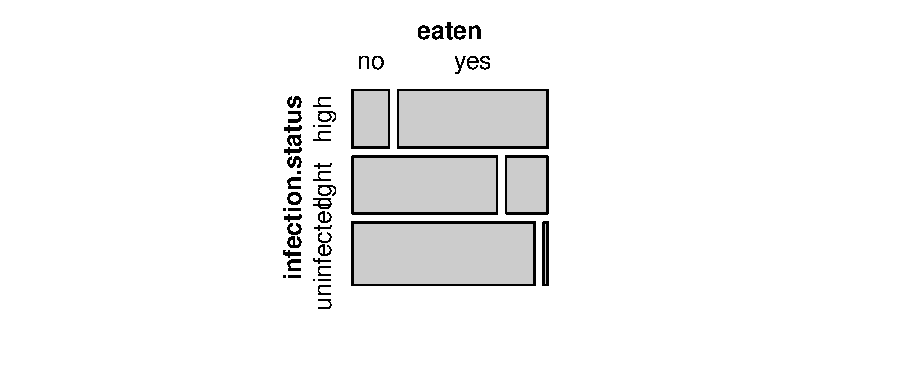
\includegraphics{figures/fig-mosaic1} 

\end{kframe}}
\end{knitrout}

\authNote{NH: this is pretty boring, but I couldn't get "sector" to display
as the second variable without major headaches}
\authNote{NH: can we standardize on either the use of mosaic (from vcd, which
has a confusing name given our package) or mosaicplot?}
\Caution{The \function{mosaic()} function has nothing to do with 
the \pkg{mosaic} package, they just happen to share the same name.}%



Alternatively, we can send \function{mosaic()} the output of \function{xtabs()}:
\begin{knitrout}
\definecolor{shadecolor}{rgb}{.97, .97, .97}{\color{fgcolor}\begin{kframe}
\begin{flushleft}
\ttfamily\noindent
\hlfunctioncall{mosaic}\hlkeyword{(}\hlfunctioncall{xtabs}\hlkeyword{(}\hlkeyword{\urltilda{}}\hlsymbol{sex}{\ }\hlkeyword{+}{\ }\hlsymbol{union}\hlkeyword{,}{\ }\hlsymbol{CPS}\hlkeyword{)}\hlkeyword{)}{\ }{\ }\hlcomment{\usebox{\hlnormalsizeboxhash}{\ }non-whites{\ }are{\ }more{\ }likely{\ }to{\ }be{\ }unionized}\mbox{}
\normalfont
\end{flushleft}
\begin{verbatim}
    union Not Union
sex                
F         217    28
M         221    68
\end{verbatim}
\end{kframe}}
\end{knitrout}

\FoodForThought{Neither \function{mosaic()} nor the similar \function{mosaicplot()}
are as clever as one could hope.  In particular, without some extra customization,
both tend to look bad if the levels of the variables have long names.
\function{mosaic()} plots also always stay square.}


Or we can send our own hand-made table (although the output isn't quite as nice without some
extra effort we won't discuss just now):
\begin{knitrout}
\definecolor{shadecolor}{rgb}{.97, .97, .97}{\color{fgcolor}\begin{kframe}
\begin{flushleft}
\ttfamily\noindent
\hlfunctioncall{mosaic}\hlkeyword{(}\hlsymbol{mycrosstable}\hlkeyword{)}\mbox{}
\normalfont
\end{flushleft}
\end{kframe}}
\end{knitrout}




\begin{problem}
The \dfn{Utilities2} data set in the \verb!mosaic! package contains a number of variables
about the utilities bills at a residence in Minnesota over a number of years.
Since the number of days in a billing cycle varies from month to month, variables 
like \vn{gasbillpday} (\dfn{elecbillpday}, etc.) contain the gas bill (electric bill, etc.) 
divided by the number of days in the billing cycle.
\begin{enumerate}
\item
Make a scatter plot of \dfn{gasbillpday} vs. \dfn{monthsSinceY2K} using the command
\begin{knitrout}
\definecolor{shadecolor}{rgb}{.97, .97, .97}{\color{fgcolor}\begin{kframe}
\begin{flushleft}
\ttfamily\noindent
\hlfunctioncall{xyplot}\hlkeyword{(}\hlsymbol{gasbillpday}{\ }\hlkeyword{\urltilda{}}{\ }\hlsymbol{monthsSinceY2K}\hlkeyword{,}{\ }\hlargument{data}{\ }\hlargument{=}{\ }\hlsymbol{Utilities2}\hlkeyword{,}{\ }\hlargument{type}{\ }\hlargument{=}{\ }\hlstring{"{}l"{}}\hlkeyword{)}{\ }{\ }\hlcomment{\usebox{\hlnormalsizeboxhash}{\ }the{\ }letter{\ }l}\mbox{}
\normalfont
\end{flushleft}
\end{kframe}}
\end{knitrout}

\item[]
What pattern(s) do you see?
\item
What does \verb!type='l'! do?  Make your plot with and without it.  Which is easier to read
in this situation?
\item
What happens if we replace 
\verb!type='l'! with 
\verb!type='b'!?
\item
Make a scatter plot of \vn{gasbillpday} by \vn{month}.   
What do you notice?

\item
Make side-by-side boxplots of \vn{gasbillpday} by \vn{month} using the \dfn{Utilities2}
data frame.   
What do you notice?

Your first try probably won't give you what you expect.  The reason is that month is coded
using numbers, so \R\ treats it as numerical data.  We want to treat it as categorical data.
To do this in \R\, use \verb!factor(month)! in place of \dfn{month}.  
\R\ calls categorical data a \term{factor}.

\item
Make any other plot you like using this data.  Include both a copy of your plot and a 
discussion of what you can learn from it.
\end{enumerate}
\end{problem}

\begin{problem}
The table below is from a study of nighttime lighting in infancy and 
eyesight (later in life).  
% latex table generated in R 2.12.1 by xtable 1.5-6 package
% Fri Feb  4 15:46:48 2011
\begin{center}
\begin{tabular}{rrrr}
  \hline
 & no myopia & myopia & high myopia \\ 
  \hline
darkness & 155 & 15 & 2 \\ 
  nightlight & 153 & 72 & 7 \\ 
  full light & 34 & 36 & 3 \\ 
   \hline
\end{tabular}
\end{center}

\begin{enumerate}
%\item
%Do you think this was an experiment or an observational study?  Why?
\item
Recreate the table in \Rstudio.  %Copy and paste the results into your Word document.
\item
What percent of the subjects slept with a nightlight as infants?

There are several ways to do this.  You could use \R\ as a calculator to do the arithmetic.
You can save some typing if you use the function \verb!prop.table()!.  See
\verb!?prop.table! for documentation.
If you just want row and column totals added to the table, see \verb!mar_table()!
in the \verb!vcd! package.
\item
Make a mosaic plot for this data.  What does this plot reveal?
\end{enumerate}
\end{problem}

Barcharts can also be used to display two-way tables.  First we convert
the cross-table to a data frame.
Then we can use this data frame for plotting.

\begin{knitrout}
\definecolor{shadecolor}{rgb}{.97, .97, .97}{\color{fgcolor}\begin{kframe}
\begin{flushleft}
\ttfamily\noindent
\hlsymbol{cps}{\ }\hlassignement{\usebox{\hlnormalsizeboxlessthan}-}{\ }\hlfunctioncall{as.data.frame}\hlkeyword{(}\hlfunctioncall{xtabs}\hlkeyword{(}\hlkeyword{\urltilda{}}\hlsymbol{sector}{\ }\hlkeyword{+}{\ }\hlsymbol{race}\hlkeyword{,}{\ }\hlargument{data}{\ }\hlargument{=}{\ }\hlsymbol{CPS}\hlkeyword{)}\hlkeyword{)}\hspace*{\fill}\\
\hlstd{}\hlsymbol{cps}\mbox{}
\normalfont
\end{flushleft}
\begin{verbatim}
     sector race Freq
1  clerical   NW   15
2     const   NW    3
3     manag   NW    6
4     manuf   NW   11
5     other   NW    5
6      prof   NW    7
7     sales   NW    3
8   service   NW   17
9  clerical    W   82
10    const    W   17
11    manag    W   49
12    manuf    W   57
13    other    W   63
14     prof    W   98
15    sales    W   35
16  service    W   66
\end{verbatim}
\end{kframe}}
\end{knitrout}

\begin{knitrout}
\definecolor{shadecolor}{rgb}{.97, .97, .97}{\color{fgcolor}\begin{kframe}
\begin{flushleft}
\ttfamily\noindent
\hlfunctioncall{barchart}\hlkeyword{(}\hlsymbol{Freq}{\ }\hlkeyword{\urltilda{}}{\ }\hlsymbol{sector}\hlkeyword{,}{\ }\hlargument{groups}{\ }\hlargument{=}{\ }\hlsymbol{race}\hlkeyword{,}{\ }\hlargument{data}{\ }\hlargument{=}{\ }\hlsymbol{cps}\hlkeyword{)}\mbox{}
\normalfont
\end{flushleft}
\end{kframe}}
\end{knitrout}


\begin{knitrout}
\definecolor{shadecolor}{rgb}{.97, .97, .97}{\color{fgcolor}\begin{kframe}


\centering{}\includegraphics{figures/fig-barchart3b} 

\end{kframe}}
\end{knitrout}




\vspace{-8mm}
\section{Additional Notes on R Syntax}


\subsection{Text and Quotation Marks}

For the most part, text in \R\ must be enclosed in either single or double quotations.  
It usually doesn't matter which you use, unless you want one or the other type of 
quotation mark \emph{inside} your text.  Then you should use the other type of 
quotation mark to mark the beginning and the end.

\begin{knitrout}
\definecolor{shadecolor}{rgb}{.97, .97, .97}{\color{fgcolor}\begin{kframe}
\begin{flushleft}
\ttfamily\noindent
\hlsymbol{text1}{\ }\hlassignement{\usebox{\hlnormalsizeboxlessthan}-}{\ }\hlstring{"{}Mary{\ }didn\usebox{\hlnormalsizeboxsinglequote}t{\ }come"{}}{\ }{\ }\hlcomment{\usebox{\hlnormalsizeboxhash}{\ }apostrophe{\ }inside{\ }requires{\ }double{\ }quotes{\ }around{\ }text}\hspace*{\fill}\\
\hlstd{}\hlsymbol{text2}{\ }\hlassignement{\usebox{\hlnormalsizeboxlessthan}-}{\ }\hlstring{"{}Do{\ }you{\ }use{\ }\usebox{\hlnormalsizeboxbackslash}"{}scare{\ }quotes\usebox{\hlnormalsizeboxbackslash}"{}?"{}}{\ }{\ }\hlcomment{\usebox{\hlnormalsizeboxhash}{\ }this{\ }time{\ }we{\ }flip{\ }things{\ }around}\mbox{}
\normalfont
\end{flushleft}
\end{kframe}}
\end{knitrout}


If you omit quotes, you will often see error messages telling you that \R\ can't find 
an object because \R\
will look for a function, data set or other object with that name instead of treating
your text as text.
\begin{knitrout}
\definecolor{shadecolor}{rgb}{.97, .97, .97}{\color{fgcolor}\begin{kframe}
\begin{flushleft}
\ttfamily\noindent
\hlsymbol{text3}{\ }\hlassignement{\usebox{\hlnormalsizeboxlessthan}-}{\ }\hlsymbol{blah}\mbox{}
\normalfont
\end{flushleft}
\begin{verbatim}
Error: object 'blah' not found
\end{verbatim}
\end{kframe}}
\end{knitrout}


\subsection{Functions}

Functions in \R\ use the following syntax:

\begin{knitrout}
\definecolor{shadecolor}{rgb}{.97, .97, .97}{\color{fgcolor}\begin{kframe}
\begin{flushleft}
\ttfamily\noindent
\hlfunctioncall{functionname}\hlkeyword{(}\hlsymbol{argument1}\hlkeyword{,}{\ }\hlsymbol{argument2}\hlkeyword{,}{\ }\hlsymbol{...}\hlkeyword{)}\mbox{}
\normalfont
\end{flushleft}
\end{kframe}}
\end{knitrout}

\vspace{-5mm}
\begin{itemize}
\item The arguments are \underline{always} \emph{surrounded by (round) parentheses} and 
\emph{separated by commas}.
\begin{itemize}
\item
Some functions (like \verb!col.whitebg()!) 
have no arguments, but you still need the parentheses.
\end{itemize}
\item
Most arguments have names, but you don't need to use the names \emph{if you 
give the arguments in the correct order}.  

If you use names, you can give the arguments out of order.  
The following do the same thing,
%\end{itemize}

\begin{knitrout}
\definecolor{shadecolor}{rgb}{.97, .97, .97}{\color{fgcolor}\begin{kframe}
\begin{flushleft}
\ttfamily\noindent
\hlfunctioncall{xyplot}\hlkeyword{(}\hlsymbol{Sepal.Length}{\ }\hlkeyword{\urltilda{}}{\ }\hlsymbol{Sepal.Width}\hlkeyword{,}{\ }\hlargument{data}{\ }\hlargument{=}{\ }\hlsymbol{iris}\hlkeyword{,}{\ }\hlargument{groups}{\ }\hlargument{=}{\ }\hlsymbol{Species}\hlkeyword{)}\hspace*{\fill}\\
\hlstd{}\hlfunctioncall{xyplot}\hlkeyword{(}\hlsymbol{Sepal.Length}{\ }\hlkeyword{\urltilda{}}{\ }\hlsymbol{Sepal.Width}\hlkeyword{,}{\ }\hlsymbol{iris}\hlkeyword{,}{\ }\hlargument{groups}{\ }\hlargument{=}{\ }\hlsymbol{Species}\hlkeyword{)}\hspace*{\fill}\\
\hlstd{}\hlfunctioncall{xyplot}\hlkeyword{(}\hlsymbol{Sepal.Length}{\ }\hlkeyword{\urltilda{}}{\ }\hlsymbol{Sepal.Width}\hlkeyword{,}{\ }\hlargument{groups}{\ }\hlargument{=}{\ }\hlsymbol{Species}\hlkeyword{,}{\ }\hlsymbol{iris}\hlkeyword{)}\mbox{}
\normalfont
\end{flushleft}
\end{kframe}}
\end{knitrout}

%\begin{itemize}
%\item[]
But these do not work
%\end{itemize}

\begin{knitrout}
\definecolor{shadecolor}{rgb}{.97, .97, .97}{\color{fgcolor}\begin{kframe}
\begin{flushleft}
\ttfamily\noindent
\hlfunctioncall{xyplot}\hlkeyword{(}\hlsymbol{Sepal.Length}{\ }\hlkeyword{\urltilda{}}{\ }\hlsymbol{Sepal.Width}\hlkeyword{,}{\ }\hlsymbol{Species}\hlkeyword{,}{\ }\hlsymbol{iris}\hlkeyword{)}\hspace*{\fill}\\
\hlstd{}\hlfunctioncall{xyplot}\hlkeyword{(}\hlsymbol{Sepal.Length}{\ }\hlkeyword{\urltilda{}}{\ }\hlsymbol{Sepal.Width}\hlkeyword{,}{\ }\hlsymbol{iris}\hlkeyword{,}{\ }\hlsymbol{Species}\hlkeyword{)}\mbox{}
\normalfont
\end{flushleft}
\end{kframe}}
\end{knitrout}

%\begin{itemize}
%\item[]
The first fails because the second argument is \verb!data!, so \verb!iris!
needs to be in the second position if it is not named.
The second fails because \verb!groups! is not the third argument.
(There are many other arguments between \verb!data! and \verb!groups! .)
The documentation for functions shows the correct order of arguments.
\item
Typically, we will not use names for the first argument or two (these tend to be 
very important arguments that have to be there) but will use names for the rest (these 
are often optional arguments that can be present or not, depending on whether we want 
the default behavior or something special).
\end{itemize}

\section{Installing R}

\subsection{RStudio in the cloud}
Our primary version of \R\ will be the online version of \Rstudio.  
You should have an \Rstudio\ account at \url{http://beta.rstudio.org/} 
using your Gmail address.
\Rstudio\ is a brand new (and quite nice) interface to \R\ that runs in a web browser.
This has the advantage that you don't have to install or configure anything.  Just login
and you are good to go.  Futhermore, \Rstudio\ will ``remember'' what you were doing so that
each time you login (even on a different machine) you can pick up right where you left off.
This is ``\R\ in the cloud" and works a bit like GoogleDocs for \R.

If you find bugs or have suggestions for \Rstudio, let us know.  It is in rapid development
at the moment, and we can pass along your feedback to the developers.  

This should be all you need for this course.  But if you prefer to have a
stand-alone version (because you study somewhere without an internet
connection, or have data that can't be loaded into the cloud, for example), read on.


\subsection{RStudio on Your Desktop/Laptop}
There is also a stand-alone version of the \Rstudio\ environment that you can install on
your desktop or laptop machine.  
This can be downloaded from \url{http://www.rstudio.org/}.  This assumes that you 
have a version of R installed on your computer (see below for instructions to download
this from CRAN).


\subsection{Getting R from CRAN}
\label{sec:CRAN}

CRAN is the Comprehensive \R\ Archive Network (\url{http://cran.r-project.org/}).  
You can download free versions of \R\ for PC, Mac, and Linux from CRAN.  (If you use
the \Rstudio\ stand-alone version, you also need to install \R\ this way first.)
All the instructions for downloading and installing are on CRAN.  Just 
follow the appropriate instructions for your platform.

\subsection{RStudio in the cloud on your own server}

At present, we are using a beta version of \RStudio\ running on their servers.  
It is also possible to install this on servers at your institution.  This will
almost certainly require a discussion with your administrators, but may be worthwhile
to facilitate student use in this manner.

\authNoted{NH: Are you both comfortable with this?}


\newpage

\section{\R\ Examples}
\vspace{-3mm}
The commands below are illustrated with the data sets \verb!iris! and 
\verb!CPS!.  To apply these in other situations, you will need to 
substitute the name of your data frame and the variables in it.

\vspace{-3mm}
\begin{center}
\begin{longtable}{p{2.45in}p{3.30in}}
\verb!answer <- 42! & Store the value 42 in a variable named \verb!answer!.
\\[3mm]
%\verb!sl <- iris$Sepal.Length! & Store the \verb!Sepal.Length! variable from the 
%\verb!iris! data frame into a variable called \verb!sl! (to save typing, for example).
%\\[3mm]
\verb!log(123); log10(123); sqrt(123)! & Take natural logarithm, base 10 logarithm, or square 
root of 123.
\\[3mm]
\verb!x <- c(1,2,3)! & Make a variable containing values 1, 2, and 3 (in that order).
\\[3mm]
\verb!data(iris)! & (Re)load the data set \verb!iris!.
\\[3mm]
%\verb!findData(2)! & Find \verb!abd! data in chapter 2.
%\\[3mm]
\verb!summary(iris$Sepal.Length)! & 
Summarize the distribution of the \verb!Sepal.Length! variable in the \verb!iris! data
frame.
\\[3mm]
\verb!summary(iris)! & 
Summarize each variable in the \verb!iris! data frame.
\\[3mm]
\verb!str(iris)! & A different way to summarize the \verb!iris! data frame.
\\[3mm]
\verb!head(iris)! & First few rows of the data frame \verb!iris!.
\\[3mm]
\verb!require(Hmisc)!

\verb!require(abd)!

\ 
& Load packages.  
(This can also be done by checking boxes in the \tab{Packages} tab.)
\\[3mm]
\multicolumn{2}{l}{
\texttt{summary(Sepal.Length\~{}Species,data=iris,fun=favstats) } 
}
\\[1mm]
& 
Compute favorite statistics of \verb!Sepal.Length! for each \verb!Species!.
[requires \verb!Hmisc!]
\\[3mm]
%\verb!cut(x,breaks,right=TRUE)! & Divide up the range of \verb!x! into 
%	intervals and code the values in \verb!x! according to which interval 
%	they fall into. 
%\\[3mm]
\multicolumn{2}{l}{\texttt{histogram(\~{}Sepal.Length|Species, iris)}}
\\[1mm]
& 
Histogram of \verb!Sepal.Length! conditioned on \verb!Species!.
\\[3mm]
\verb!bwplot(Sepal.Length~Species, iris)! & 
Boxplot of \verb!Sepal.Length! conditioned on \verb!Species!.
\\[3mm]
\multicolumn{2}{l}{\texttt{xyplot(Sepal.Length\~{}Sepal.Width|Species, iris)}} 
\\[1mm]
& 
Scatterplot of \verb!Sepal.Length! by \verb!Sepal.Width! 
with separate panels for each  \verb!Species!.
\\[3mm]
\verb!xtabs(~sector, CPS)! & Frequency table of the variable \verb!sector!.
\\[3mm]
\multicolumn{2}{l}{\texttt{barchart(xtabs(\~{}sector, CPS))}}
\\[1mm]
& Make a barchart from the table.
\\[3mm]
\multicolumn{2}{l}{\texttt{xtabs(\~{}sector + race, CPS)}}
\\[1mm]
& Cross tabulation of \verb!sector!  and \verb!race!.
\\[3mm]
\multicolumn{2}{l}{
\texttt{mosaic(\~{}sector + race, CPS)} }
\\[1mm]
& Make a mosaic plot.
\\[3mm]
\multicolumn{2}{l}{
\texttt{xtData <- as.data.frame( xtabs(\~{}sector + race, Trematodes) )}}
\\[1mm]
  & Save cross table information as \verb!xtData!. 
\\[3mm]
\multicolumn{2}{l}{
\texttt{barchart(Freq\~{}sector, data=xtData, groups=race)}
}
\\[1mm]
& Use \verb!xtData! to make a segmented bar chart.
\\[3mm]
\verb!sum(x)!; 
\verb!mean(x)!; 
\verb!median(x)!;

\verb!var(x)!; 
\verb!sd(x)!; 
\verb!quantile(x)!
& Sum, mean, 
median,
variance,
standard deviation,
quantiles of \verb!x!.
\\
\end{longtable}
%\rule{4in}{1pt}
\end{center}

\vspace*{-.5in}
\section{Exercises}

%For these problems, create a single Word document containing all of your work.

\shipoutProblems


